\documentclass{article}

\usepackage[spanish]{babel}
\hyphenation{i-rra-dia-dor}
\usepackage[utf8]{inputenc}
\usepackage[backend=bibtex,sorting=none]{biblatex}
\bibliography{bibliografia.bib}
\usepackage{etoolbox}
%\usepackage{todonotes}
%\robustify{\today}
\usepackage[]{hyperref}
%\hypersetup{pdftex,colorlinks=true,allcolors=blue}
\hypersetup{pdfpagemode=UseOutlines}
%\usepackage{hypcap}
\usepackage{amssymb}
\usepackage[]{amsmath}
\usepackage[]{mathrsfs}
\usepackage{graphicx}
\usepackage{float}
\usepackage{caption}
\usepackage{subcaption}
\usepackage[load=addn]{siunitx}
\usepackage{textcomp}

\graphicspath{ {imagenes/} }
\newcommand{\figref}[1]{figura~\ref{#1}}
\newcommand{\equref}[1]{ecuación~\ref{#1}}
% \fig{label}{archivo}{caption}
\newcommand{\fig}[3]{
\begin{figure}[H]
    \centering
    %\includegraphics[width=\columnwidth]{#2}
    \includegraphics{#2}
    \caption{#3}
    \label{fig:#1}
\end{figure}}
\newcommand{\figp}[3]{
\begin{figure}[p]
    \centering
    %\includegraphics[width=\columnwidth]{#2}
    \includegraphics{#2}
    \caption{#3}
    \label{fig:#1}
\end{figure}}
\newcommand{\cita}[1]{\cite{#1}}
\newcommand{\deriv}[2]{\frac{d#1}{d#2}}
\newcommand{\pderiv}[2]{\frac{\partial#1}{\partial#2}}
\newcommand{\strontium}{\mathrm{Sr}}
\newcommand{\isotope}[2]{\ensuremath{\left.^{#2}\mathrm{#1}\right.}}
\newcommand{\Strontium}{\ensuremath{\left.^{90}\mathrm{Sr}\right.}}
\newcommand{\yttrium}{\mathrm{Y}}
\newcommand{\Yttrium}{\ensuremath{\left.^{90}\mathrm{Y}\right.}}
\newcommand{\zirconium}{\mathrm{Zr}}
\newcommand{\vdd}{\ensuremath{V_{\text{DD}}}}
\def\code#1{\texttt{#1}}

\author{Ignacio Martinez Vazquez}
\date{}

\begin{document}
\begin{titlepage}
   \begin{center}
\vspace*{1cm}

\Huge
\textbf{Non-conventional MOS dosimeters: design, fabrication and characterization}

\vspace{0.5cm}
 
\vspace{1.5cm}
 
\Large
\textbf{Ignacio Martinez Vazquez}

\vfill

Physics Licentiate Thesis\\
Facultad de Ciencias Exactas y Naturales\\
Universidad de Buenos Aires\\
 
       \vspace{0.8cm}
 
   \end{center}
\end{titlepage}
%
\textbf{Title:} Non-conventional MOS dosimeters: design, fabrication and characterization

\textbf{Student:} Ignacio Martinez Vazquez 

\textbf{Research group:} Laboratorio de Física de Dispositivos - Microelectrónica (FIUBA)

\textbf{Advisor:} Dr. Adrián Faigón

\textbf{Submission date:} Diciembre de 2018

\vfill
\newpage

\tableofcontents
\listoffigures
\clearpage
\part*{Agradecimientos}
Agradezco a todos los que hicieron posible este trabajo:
\begin{itemize}
    \item Laboratorio de Física de Dispositivos - Microelectrónica: 
    por toda la enseñanza, guía y oportunidades brindadas.
    Especialmente Mariano por cargar la fuente en el irradiador.
    \item Eriel Fernandez y todo el taller mecánico de FIUBA: 
    por los trabajos y piezas con que aportaron a la construcción del
    irradiador, y por la ayuda en definir los mecanismos.
    \item Abraham Murillo y la Escuela Técnica Nº 33 Fundicion Maestranza del 
    Plumerillo:
    por el planeamiento y realización de la fundición en plomo para el
    irradiador.
    \item Iván G. Pollitzer y el Laboratorio Abierto de Electrónica:
    por la impresión 3D para el irradiador
    \item Universidad de Buenos Aires:
    por la beca estímulo.
    \item CITEDEF: por el wire-bonding de los circuitos fabricados.
\end{itemize}
\clearpage

\section{Introducción}
Luego del descubrimiento de los rayos X,
la radiación se convirtió en una herramienta
que acumuló numerosas aplicaciones médicas e industriales.
Paralelamente,
se empezó a tomar conciencia de 
los peligros de la exposición a la radiación
y la importancia de cuantificar la dosis que recibe una persona.

Hoy en día,
más y más técnicas médicas de diagnóstico y terapia
exponen al paciente a distintas formas de radiación.
El control de la dosis se logra mediante calibración de la maquinaria
y cálculos Monte Carlo para modelar la propagación de la radiación.

Midiendo la dosis administrada a cada parte del paciente
se reduce enormemente este riesgo.
Al mismo tiempo,
abre la puerta a terapias más efectivas:
es posible planificar cada sesión de radiación
en respuesta al resultado de la anterior,
corrigiendo por fallas de alineamiento, calibración y cambios en el
paciente\cite{wu_application_2006}.

Para obtener esa información hacen falta dosímetros 
que se presten al uso médico.
Esto pasa tanto por sus especificaciones técnicas
(sensibilidad, dosis máxima)
como por su costo,
biocompatibilidad y tamaño.
Un grupo muy prometedor de dosímetros usa técnicas 
provenientes de la fabricación de circuitos integrados 
para obtener dosímetros fácilmente
miniaturizables\cite{holmes-siedle_radfet:_1986}.
Actualmente consisten en circuitos que miden el corrimiento de parámetros de un transistor
especialmente sensible a la radiación, debido a su óxido de compuerta muy
grueso.

Dentro de los dosímetros integrables 
(que se pueden incorporar con otras funciones en un circuito integrado),
hay gran interés en aquellos fabricados usando, sin modificación,
procesos comerciales para circuitos integrados\cite{lipovetzky_field_2013}
\cite{wang_temperature_2005}
\cite{garcia-moreno_floating_2012}
\cite{dulinski_cmos_2004}.
Esto quita la posibilidad de optimizar y controlar 
muchos parámetros del proceso.
A cambio de esa restricción, 
permite integrar circuitería adicional
para procesamiento de señales e interfaz con el mundo exterior,
aprovechando las economías de escala de los procesos estándar.

En este trabajo diseñamos, construímos y caracterizamos
dos dosímetros fabricados en un proceso estándar CMOS de
\SI{0.6}{\micro\meter}.
El primero es un Active Pixel Sensor,
de estructura similar a un pixel del sensor de una cámara digital:
tiene un diodo polarizado en inversa, con una zona desierta de portadores.
La radiación incidente en esta zona genera pares electrón-hueco.
El campo eléctrico separa electrones de huecos,
y la baja concentración de portadores aumenta su tiempo de vida permitiendo
recolectarlos.
Su ventaja sobre dosímetros tradicionales es la capacidad de resetearlo
instantáneamente de manera electrónica,
simplemente descargando el capacitor que acumula la carga generada por
radiación.

El segundo es un Floating Gate,
semejante a una celda de una memoria Flash.
Aquí la radiación genera carga en el aislante que rodea la compuerta de un
transistor MOS.
Este dispositivo es ideal para sensar esa carga acumulada:
en condiciones normales, la corriente de compuerta es despreciable 
y no descarga al nodo donde se está acumulando la carga.
Este dosímetro se destaca por la posibilidad de medir radiación sin suministro de tensión.

Ambos dosímetros explotan la respuesta a radiación de estructuras 
normalmente utilizadas para otros fines. 
Luego de una introducción a la teoría de su funcionamiento,
presentamos el proceso y las consideraciones de diseño,
y los resultados de las mediciones de ambos dosímetros 
comparando con los valores calculados.

\part{Teoría}
\section{Fundamentals of Metal Oxide Semiconductor structures}
MOS structures are the basis for modern integrated circuits
\cita{sze_physics_2007}
which make up PCs, mobile devices and communication infrastructure.
The CMOS fabrication process which produces these structures
has enabled processing power to grow exponentially,
by steadily shrinking the transistors that make up an integrated circuit
(\figref{fig:moore}).
\fig{moore}{figuras/moore/moore.pdf}
{Exponential reduction in transistor size.
The number of transistors in a microprocessor doubles every two years,
following Moore's law
\cite{moore_cramming_2006}.
Reprinted from \cite{sedra_microelectronic_2010}.}
\subsection{MOS capacitor}
Before studying MOS transistors, it is necessary to understand MOS capacitors.
Fabrication begins with a ~\SI{1}{\milli\meter} silicon wafer cut from a monocrystalline ingot.
Its surface is oxidized in order to produce a thin insulating SiO$_2$ layer.
Both this step and subsequent treatment and annealing steps
determine a crucial property of the Si-SiO$_2$ interface:
the surface density of electronic states.
If this number is too large, the device characteristics are negatively impacted:
for example, through higher noise and parameter shifts over time.
The invention that improved interfaces and thus enabled decent MOS transistors
came decades after the MOS was originally patented
\cite{chih-tang_evolution_1988}.

On top of the oxide layer, a conductor (gate) is deposited,
as seen in \figref{fig:cortemos}.
This conductor can be polysilicon (polycrystalline silicon) or,
in recent processes, metal.
\fig{cortemos}{figuras/mos/corte.png}{Cross section of a MOS structure.
Reprinted from~\cite{sze_physics_2007}.}

This structure forms a capacitor, with two conductors separated by a dielectric.
%
\subsubsection{Band structure}
The following analysis assumes a MOS whose dimensions along the wafer
are much larger than the characteristic distance 
across which the electric field varies normal to the wafer.
This allows us to use a 1D model,
neglecting field variations parallel to the wafer.

The ideal MOS band structure is depicted in \figref{fig:bandasmos}.
An ideal MOS has no charge trapped in the oxide nor in the oxide-semiconductor interface.
Therefore, its bands are flat under zero bias.
We will analyze how band position varies with applied bias and with distance from the wafer surface.

When a voltage source (eg. a battery) is connected across the terminals,
it fixes the difference between the Fermi levels of the metal and the semiconductor.
The resulting $E_F$ gradient leads to a current within the MOS which restores equilibrium
(\figref{fig:polarizacionmos}).

%Bajo la condición $V=0$, los niveles de Fermi de metal y
%semiconductor coinciden.
%Para cada material, el nivel de vacío $\phi$ 
%está a una distancia fija del nivel de Fermi.
%En un metal esta distancia se denomina función trabajo.
%En un semiconductor esta cantidad es la suma de la afinidad electrónica $\xi$
%(distancia entre la banda de conducción y el nivel de vacío)
%y 
%Por ejemplo, la función trabajo del aluminio es \SI{4.2}{\volt} y la de una
%oblea dopada tipo P típica es \SI{3.6}{\volt}.
%Cuando coinciden los niveles de Fermi de metal y semiconductor, 
%difiere su potencial eléctrico en \SI{0.6}{\volt}.
%$\phi$ varía de forma contínua entre las terminales,
%curvando las bandas.
%Hace falta aplicar una tensión $V_{fb}=(\phi_m-\phi_s)/e$ 
%para obtener bandas planas (que implican, por Poisson, carga nula).
%
\fig{bandasmos}{figuras/mos/bandas.png}
{Band structure of a MOS capacitor in the flatband condition.
Reprinted from~\cite{sze_physics_2007}.}
\begin{figure}[H]
    \centering
    \begin{subfigure}[b]{.3\textwidth}
        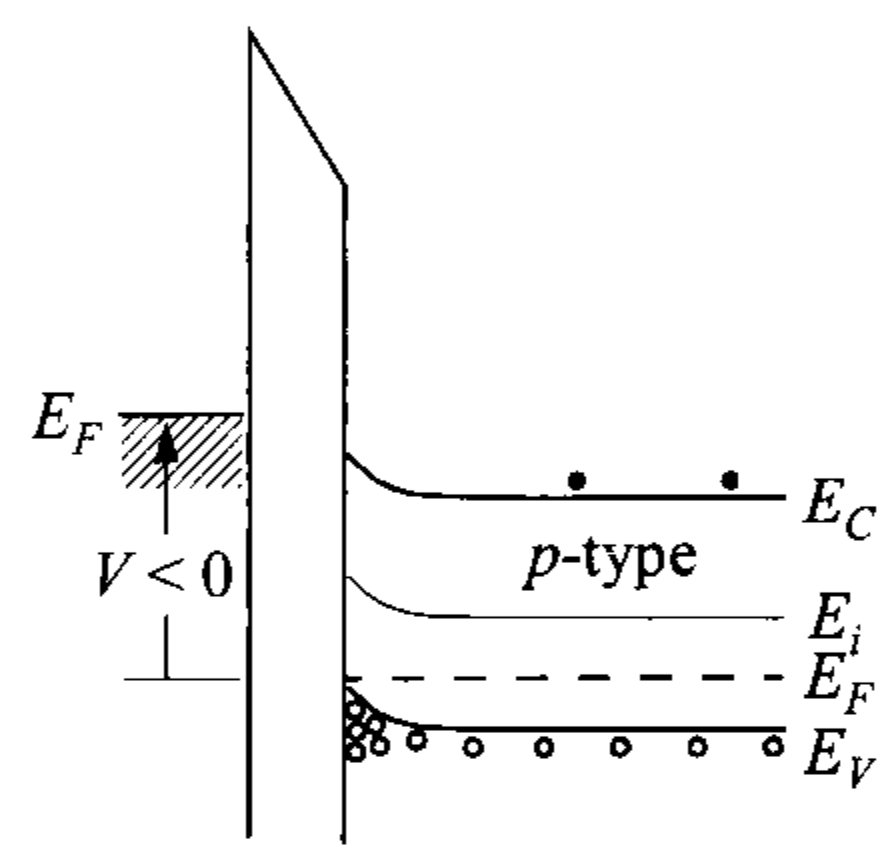
\includegraphics{figuras/mos/acumulacion.png}
        \label{fig:mosacumulacion}
        \caption{Accumulation}
    \end{subfigure}
    \begin{subfigure}[b]{.3\textwidth}
        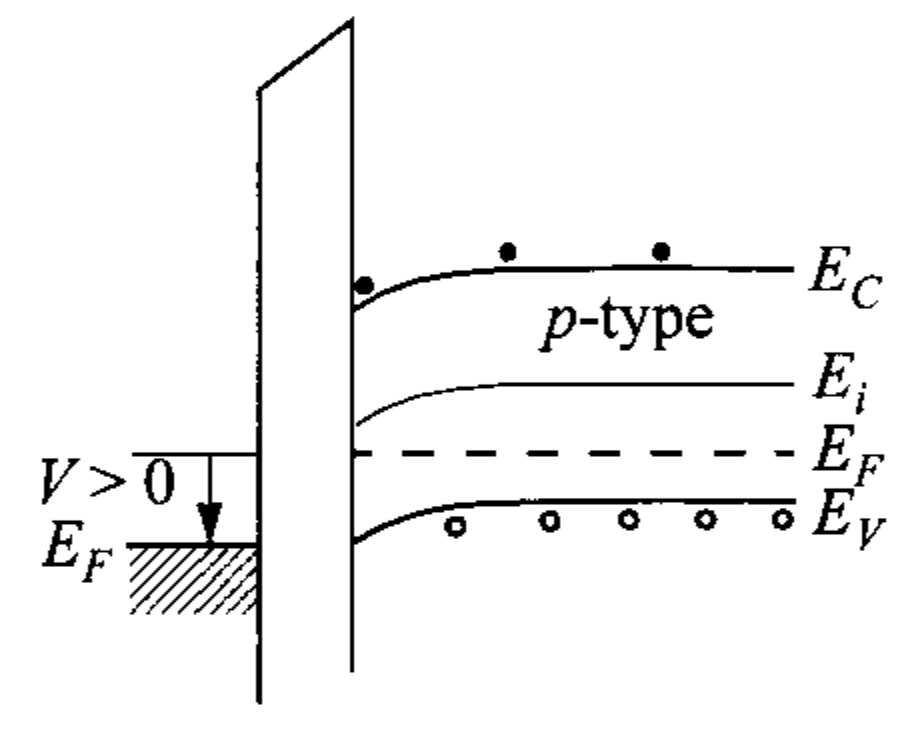
\includegraphics{figuras/mos/desercion.png}
        \label{fig:mosdesercion}
        \caption{Deserción}
    \end{subfigure}
    \begin{subfigure}[b]{.3\textwidth}
        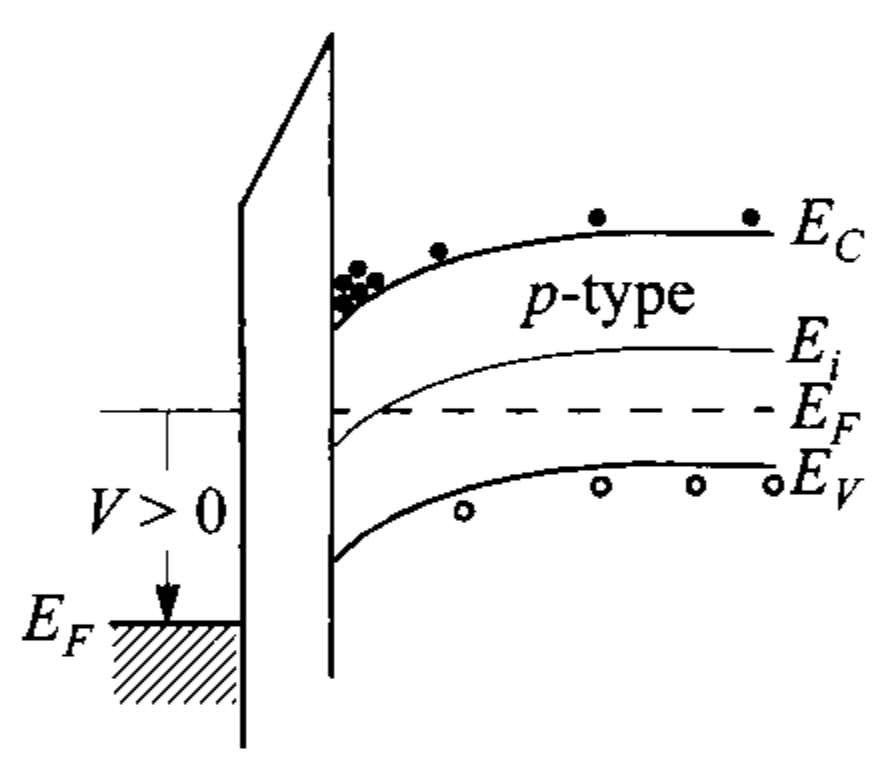
\includegraphics{figuras/mos/inversion.png}
        \caption{Inversión}
        \label{fig:mosinversion}
    \end{subfigure}
    \caption{Bandas del MOS polarizado, para $V_{fb}=0$.
Reproducido de~\cite{sze_physics_2007}.}
    \label{fig:polarizacionmos}
\end{figure}
%
\subsubsection{Concentración de portadores}
Para modelar la concentración de huecos y electrones en semiconductores,
se parte de la aproximación de electrón independiente.
La misma permite pensar en términos de niveles de 1 electrón que son ocupados
por electrones idénticos que no interactúan.
La termodinámica de un sistema así
lleva a la estadística de Fermi-Dirac, 
que dice que la probabilidad de ocupación de un nivel está dada por
\begin{align*}
    f(E) = \left[\exp\left(\frac{E-E_F}{kT}\right)+1\right]^{-1}
\end{align*}
con $E$ la energía del nivel y $E_F$ el nivel de Fermi.
$E_F$ es constante a lo largo de un sistema en equilibrio
químico,
y puede despejarse como función del número total de partículas.
Para eso se invierte la identidad $N=\sum_E f(E)$ donde la suma es sobre
todos los niveles de energía.

Para obtener la cantidad promedio de portadores en una banda,
es necesario sumar la ocupación de todos los niveles de la misma. 
En muchos casos de interés la banda de conducción cumple 
$|E-E_F| \gg kT$.
Esto permite aproximar la distribución Fermi-Dirac 
por una distribución Maxwell-Boltzmann,
\begin{align*}
    f(E) \approx \exp\left(-\frac{E-E_F}{kT}\right)
\end{align*}.
Asimismo la suma de $f(E)$ sobre los niveles de la banda se puede aproximar
por una integral, y así se llega a las concentraciones de electrones y huecos
\begin{align*}
    n_c = N_c(T)e^{-\frac{\epsilon_c-E_F}{k_BT}}\\
    p_v = P_v(T)e^{-\frac{E_F-\epsilon_v}{k_BT}}
\end{align*} con $N_c(T)$ y $P_v(T)$ funciones que varían lentamente con la
temperatura.

Es conveniente expresar la concentración de portadores 
como función del potencial medido respecto del contacto de bulk
(un punto alejado del semiconductor, que tomamos como referencia):
$\psi_p=\phi(x)-\phi(\infty)$,
\begin{align}
    n &= n_0\exp\left(\frac{q\psi_p}{kT}\right)&
    p &= p_0\exp\left(-\frac{q\psi_p}{kT}\right),
    \label{eq:portadores_nodegenerados}
\end{align}
con $n_0$ y $p_0$ las concentraciones de portadores en el bulk.
\subsubsection{Impurezas}
Una parte central del proceso de fabricación
es introducir impurezas que aportan electrones o huecos
en regiones cuidadosamente controladas (\emph{doping}).
Así se crean zonas con concentraciones particulares de portadores.
La geometría y concentración de cada zona
es lo que define cada tipo de dispositivo 
que un proceso es capaz de producir.
Por ejemplo, un proceso puede estar diseñado para altas tensiones
eligiendo concentraciones bajas y separaciones grandes
que logren una alta tensión de ruptura de las junturas.

Una técnica, llamada Chemical Vapor Deposition,
es exponer el sustrato a un gas
para que haya difusión de átomos del gas al sustrato.
La otra, llamada implantación, es ionizar las impurezas 
y acelerarlas mediante campos eléctricos hacia el sustrato.
Allí penetran hasta una profundidad que puede controlarse 
variando su energía\cite{campbell_science_2001}.


La forma en que las impurezas introducen portadores 
es capturando o emitiendo electrones.
Esto deja al átomo de impureza ionizado.
Para analizar este fenómeno se modela al efecto 
de una impureza con valencia 5
(uno más que el Silicio)
como si fuera un átomo normal de la red 
sumado a una carga fija +1, y un electrón.
Esta carga fija es capaz de atraer y formar estados ligados con electrones.
Usando la ecuación de masa efectiva\cite{datta_quantum_1989},
% FIXME: feo
se llega a que la energía de ligadura es muy baja
y por lo tanto las impurezas están casi totalmente ionizadas 
bajo condiciones normales de temperatura.
Esto se debe al efecto de la red: 
Por un lado actúa como dieléctrico
y apantalla el campo eléctrico de la carga.
Por otro lado altera la masa efectiva de los electrones 
y reduce la energía cinética y por lo tanto la potencial.

El análisis de impurezas aceptoras es análogo al de las donantes, 
con una carga fija -1 que se ioniza y libera un hueco.

Típicamente se dopa una región con muchas más impurezas de un tipo
que de otro: la diferencia suele ser de órdenes de magnitud.
Se dice entonces que ahí los electrones o bien los huecos 
son el portador mayoritario.
De forma equivalente, se dice que esa región es de tipo 
``P'' (dopada con aceptores) o de tipo ``N'' (dopada con donantes).
En este caso la concentración del portador mayoritario
es aproximadamente igual a la concentración de su impureza.
La concentración del otro portador se encuentra fuertemente suprimida
debido al principio de Le Chatelier,
y vale aproximadamente $n_i^2/N_a$ 
con $n_i$ la concentración de portadores del semiconductor intrínsico (puro),
y $N_a$ la concentración de la impureza mayoritaria.

\subsubsection{Relación carga-tensión}
Planteando la ecuación de Poisson para el potencial $\phi$ en el semiconductor se llega a
\begin{align*}
    \deriv{^2\phi}{x^2} &= \frac e{\epsilon_s}(N_d-N_a+p-n),
\end{align*}
siendo los términos de la derecha concentraciones de donantes, aceptores,
huecos y electrones.


La aproximación~\ref{eq:portadores_nodegenerados} es válida para 
$|E_F-E_{c/v}|\gg kT$, 
o sea el nivel de Fermi alejado de los bordes de las bandas.
Así se obtiene un sistema de ecuaciones cuya solución para el campo eléctrico es
\begin{align*}
    \mathscr{E}_s &= \pm \frac{\sqrt 2kT}{qL_D}
    F(q\psi_p/kT,n_{p0}/p_{p0})\textnormal{, con}\\
    L_D^2&=\frac{kT\epsilon_s}{p_{p0}q^2}\textnormal{ , y}\\
    F(x,y) &= \sqrt{e^{-x}+x-1+y(e^x-x-1)}.
\end{align*}
Usando la ley de Gauss se obtiene la carga total del semiconductor
\begin{align*}
    Q_s = -\epsilon_s\mathscr{E}_s.
\end{align*}
La relación entre $V_G$ y $\psi_p$ viene de plantear la continuidad del vector
desplazamiento y la caída de tensión en el aislante
\begin{align}
    V_G &= \psi_s + \mathscr{E}\frac{\epsilon_s}{\epsilon_{ox}}t_{ox}.
    \label{eq:potencial_campo_mos}
\end{align}
Esto resulta en el gráfico de la \figref{fig:cargamos},
donde delimitamos distintos regímenes de operación.
%
\subsubsection{Regímenes de operación del capacitor MOS}
\begin{itemize}
    \item Acumulación:
        Aplicando tensión negativa al gate
        se puebla la superficie de portadores mayoritarios.
    \item Flatband/bandas planas: 
        A \SI{0}{\volt} la carga positiva de los huecos 
        (portadores mayoritarios)
        cancela la carga negativa de los aceptores, 
        entonces $Q=0$. 
    \item Deserción/Inversión débil:
        Aumentando la tensión se vacía la superficie de portadores
        mayoritarios,
        dejando la carga neta negativa de los aceptores ionizados.
    \item Inversión fuerte:
        Al cruzar $2\psi_B$ se puebla la superficie de portadores minoritarios
        con carga negativa,
        de igual magnitud y signo opuesto a la del sustrato.
        Un pequeño aumento adicional de $\psi_s$ resulta en un aumento exponencial
        de $|Q|$.
        Esta dependencia exponencial es válida hasta que el nivel de Fermi 
        se aproxima al borde de la banda de conducción y 
        el semiconductor se torna degenerado.
        Esto significa que se comporta como un metal,
        con una densidad de portadores que varía lentamente con el potencial.
        Antes de este punto, la carga pasa a crecer linealmente con $V_G$
        porque casi toda la tensión adicional cae a través del óxido de gate.
\end{itemize}
\fig{cargamos}{figuras/mos/carga_vg.pdf}{Carga de un MOS típico 
    ($N_A=$\SI{4e15}{\centi\meter^{-3}}) en función
de la tensión de gate.
En la región de la izquierda el nivel de Fermi se acerca a la banda de
valencia. Esto torna degenerado al semiconductor y requiere el uso de
estadística de Fermi-Dirac en vez de aproximarla por Maxwell-Boltzmann.}
%
%
\subsection{Transistor MOS}
El transistor es la base de la electrónica moderna.
Modulando una señal con otra, 
permite realizar operaciones analógicas como amplificación y multiplicación.
Al operarlo con niveles discretos (prendido/apagado),
permite realizar las operaciones lógicas básicas (NOT, AND, etc.) que
se combinan para formar un circuito digital.
Su evolución permitió la integración de un número creciente de funciones
digitales y analógicas en un mismo circuito integrado.
%
\subsubsection{Modelo circuital}
\label{section:ecuaciones_mos}
El MOSFET o transistor MOS es un dispositivo con 4 terminales:
drain, gate, source y body (\figref{fig:mosfetschem}).
\fig{mosfetschem}{figuras/mos/mosfet.pdf}{Símbolo esquemático del transistor MOS.}
Frecuentemente se conecta source con body, rompiendo la simetría source-drain.
La tensión entre gate y source controla la corriente drain-source.

En la \figref{fig:mosfetoutput} se ven los 3 modos de operación del MOS:
\fig{mosfetoutput}{figuras/mos/output.pdf}{Curvas características de un
transistor MOS típico.}
\begin{itemize}
    \item Corte: Si $V_g<V_T$, no fluye corriente de drain.
        Por eso $V_T$ es denominada la ``tensión umbral''.
        $V_T$ es un parámetro de fabricación que ronda \SI{.3}{\volt} en procesos CMOS
        modernos.
        Un modelo más preciso es que $I_d$ depende exponencialmente de $V_g$.
    \item Triodo: Si $V_g>V_T$ y $V_{ds}<V_g-V_T$, la corriente de drain crece con la
        tensión drain-source siguiendo
        \begin{align*}
            I_D&=\beta_n\frac WL(V_{gs}-V_T-\frac{V_{ds}}2)V_{ds},
        \end{align*}
        con $\beta_n$ un parámetro del proceso y $\frac WL$ la relación de
        aspecto del MOSFET.
    \item Saturación: Si $V_g>V_T$ y $V_{ds}>V_g-V_T$ la corriente se mantiene, a primer
        orden, al valor constante
        \begin{align*}
            I_{Dsat}&=\frac{\beta_n}2\frac WL(V_{gs}-V_T)^2.
        \end{align*}
\end{itemize}
%
\subsubsection{Modelado físico}
El MOSFET de canal n consiste en un capacitor MOS de sustrato p entre dos regiones fuertemente dopadas 
tipo n, 
que forman drain y source (\figref{fig:mosfetestructura}).
Sin tensión de gate no puede fluir corriente entre drain y source porque una de las
junturas p-n (drain-sustrato o source-sustrato) queda polarizada en inversa.

Al polarizar el MOS en inversión se forma junto al óxido de gate 
una capa de electrones libres llamada canal.
Esta región de tipo n conecta drain y source y permite el flujo de corriente.
Al variar la tensión de gate, la variación de carga en el canal modula su
conductividad.
\fig{mosfetestructura}{figuras/mos/mosfet.png}{Estructura del transistor MOS.
Reproducido de~\cite{sze_physics_2007}.}

\section{Radiación}
\label{sec:radiacion}
La radiación es el transporte de energía mediado por distintas partículas.
En nuestro caso tratamos con fotones (rayos X) y electrones (rayos $\beta$).
Por encima de cierto umbral de energía, 
las interacciones de estas partículas con la materia
son capaces de ionizarla.
Esto produce daños tanto en tejidos orgánicos como en circuitos electrónicos.
%
\subsection{Radiación $\alpha$}
Las partículas $\alpha$ son núcleos de $^4$He.
Son producidas por núcleos inestables como
$^{241}$Am (usado en detectores de humo) y U 
cuando sufren decaimiento $\alpha$.
Este proceso genera partículas con energías cercanas a 
\SI{5}{\mega\electronvolt},
que se detienen en algunos centímetros de aire 
o en la capa de células muertas de la epidermis.
No son una fuente significativa de dosis a humanos,
salvo en caso de inhalación o ingestión,
o de tener energías altas
(por ejemplo si provienen de rayos cósmicos).
\subsection{Neutrones}
Los neutrones son partículas neutras presentes en los núcleos atómicos.
Los distintos isótopos de cada elemento corresponden a núcleos que difieren
sólo en la cantidad de neutrones.
Los procesos de fusión y fisión nuclear 
tienden a emitir neutrones energéticos o,
en procesos de nucleosíntesis,
capturar neutrones para formar núcleos más masivos.

A fines de protección, se estudian 3 tipos de interacciones entre neutrones
y los núcleos de un blanco:
scattering elástico e inelástico, y captura.
En el scattering inelástico,
parte de la energía inicial excita el núcleo del blanco y es luego emitida como
fotones.
La captura se da en los neutrones de menor energía,
frenados previamente por scattering,
y está acompañada por emisión de rayos $\gamma$.
Por ejemplo, en la terapia por captura neutrónica con Boro,
se hace llegar boro a células cancerígenas para que capture neutrones.
Así los tumores son destruídos por los fotones $\gamma$ y las partículas 
$\alpha$ resultantes del proceso de captura.
\subsection{Radiación $\beta$}
La radiación $\beta$ consiste en electrones energéticos.
Los mismos pasan por la materia y depositan energía por procesos de ionización 
o la emiten como radiación de frenado (bremsstrahlung).
Esto limita su rango o profundidad a la que pueden penetrar un material antes
de agotar su energía.
En aire recorren distancias típicas de metros, 
mientras que en materiales más densos recorren milímetros.

La materia con la que interactuamos tiene una gran fracción de electrones 
(en número).
Sin embargo, estos electrones se encuentran ligados a protones y neutrones,
incapaces de escapar por falta de energía.
Cuando incide radiación $\beta$ o $\gamma$ sobre un material,
puede producir electrones libres (radiación $\beta$ secundaria)
suponiendo que la partícula incidente supera la energía de ionización del
material.

Otra forma de producir radiación $\beta$ es crear nuevos electrones a partir de
energía.
Esto se da naturalmente en algunos isótopos radioactivos en un proceso llamado
decaimiento $\beta$.
\subsubsection{Decaimiento $\beta$}
El decaimiento $\beta$ es un proceso
que convierte un núcleo $X$ en otro menos masivo $X'$ y emite
un antineutrino electrónico y un electrón.
Por ejemplo, el decaimiento del estroncio a itrio
\begin{align*}
    \left.^{90}\strontium\right.
    &\to\left.^{90}\yttrium\right.+e^-+\overline\nu_e.
\end{align*}
La variación de la cantidad de átomos $N_X$ puede modelarse con
\begin{align*}
    \deriv{N_X}t &= -\lambda N_X\\
    \deriv{N_{X'}}t &= \lambda N_X
\end{align*}
si $X'$ es estable. 
$\lambda$ es un parámetro que determina la tasa de decaimiento.
La solución es
\begin{align}
    \label{eq:soluciondecaimiento}
    N_X(t) &= N_X(0)e^{-\lambda t}\\
    N_{X'}(t) &= N_X(0)(1-e^{-\lambda t}).\nonumber
\end{align}
En vez de $\lambda$ se habla comunmente de la vida media de $X$:
el tiempo $\tau$ que tarda $N_X$ en caer a la mitad.
Puede despejarse de la \equref{eq:soluciondecaimiento}
\begin{align*}
    \frac 1 2 N_X(0) &= N_X(0)e^{-\lambda\tau}\\
    \tau &= \frac{\ln2}\lambda
\end{align*}
\subsubsection{Equilibrio secular}
El nuevo núcleo creado por decaimiento $\beta$ puede, a su vez, ser inestable.
Por ejemplo, el $^{90}\strontium$ decae en $^{90}\yttrium$ que decae
en $^{90}\zirconium$.
Modelamos esto con
\begin{align*}
    \deriv{N_\strontium}t &= -\lambda_\strontium N_\strontium\\
    \deriv{N_\yttrium}t &= \lambda_\strontium N_\strontium
        -\lambda_\yttrium N_\yttrium\\
    \deriv{N_\zirconium}t &= \lambda_\yttrium N_\yttrium.
\end{align*}
Su solución es
\begin{align*}
    N_\strontium(t) &= N_\strontium(0)e^{-\lambda_\strontium t}\\
    %\deriv{N_\yttrium}t +\lambda_\yttrium N_\yttrium &= 
        %\lambda_\strontium N_\strontium(0)e^{-\lambda_\strontium t}
    N_\yttrium(t) &= ae^{-\lambda_\yttrium t}
        +N_\strontium(0)\frac{\lambda_\strontium}
        {\lambda_\yttrium-\lambda_\strontium}e^{-\lambda_\strontium t}.
\end{align*}
Dado que la vida media del $^{90}\yttrium$ (2.7 días) 
es mucho menor que la del $^{90}\strontium$ (29 años),
tenemos $\lambda_\yttrium\gg\lambda_\strontium$.
Las cantidades de cada elemento tienden a un equilibrio secular dado por
\begin{align*}
    N_\strontium(t) &= N_\strontium(0)e^{-\lambda_\strontium t}\\
    N_\yttrium(t) &\approx N_\strontium(0)
        \frac{\lambda_\strontium}{\lambda_\yttrium}
        e^{-\lambda_\strontium t}.
\end{align*}La frecuencia con que cada elemento emite un electrón es su
actividad. 
Se expresa en Becquerel
(\SI{1}{\becquerel}=\SI{1}{\per\second}) o Curie
(1 Ci=\SI{3.7e10}{\per\second}), y está dada en este ejemplo por
\begin{align*}
    A_\strontium(t) &= N_\strontium(0)\lambda_\strontium
        e^{-\lambda_\strontium t}\\
    A_\yttrium(t) &\approx N_\strontium(0)
        \frac{\lambda_\strontium}{\lambda_\yttrium}\lambda_\yttrium
        e^{-\lambda_\strontium t}=A_\strontium(t).
\end{align*}
Por lo tanto, una fuente de $^{90}\strontium$ en equilibrio secular
debe mitad de su actividad a decaimientos $\strontium\to\yttrium$
y mitad a $\yttrium\to\zirconium$.
%
\subsubsection{Frenado de electrones}
La pérdida de energía de los electrones se debe a interacciones discretas con
los átomos de un escudo.
Aproximando el frenado como una variación contínua de su energía 
en función de la distancia $E(x)$,
podemos plantear un poder de frenado $S(E)$ del material tal que
\begin{align*}
    \frac{dE}{dx}=-S(E).
\end{align*}
Se llama poder de frenado de masa a $S/\rho$. 
Esta es una medida de uso común en protección de radiación,
que permite calcular tasa de dosis de un haz usando
\begin{align*}
    \dot D&=\deriv{E}{mdt}=\frac 1\rho\deriv{E}{x}\deriv{N}{Adt}=\frac{IS}\rho
\end{align*}
con $I$ el flujo de partículas por unidad de área (intensidad)
y $\dot D$ la deposición de energía por unidad de masa y de tiempo 
(tasa de dosis).
$S$ está tabulada para cada elemento (\figref{fig:stopping})
\fig{stopping}{figuras/rad/stopping.pdf}{Poder de frenado de electrones 
para distintos materiales en función de la energía.
Valores publicados por NIST en el proyecto ESTAR\cite{berger_estar_????}.}
junto con el rango o distancia de frenado
\begin{align*}
    R(E) &= \int_0^E \frac{dE'}{S(E')}
\end{align*} y la eficiencia radiativa $Y$.
Esta es la fracción de la energía electrónica que se 
emite como fotones (\emph{bremsstrahlung} o radiación de frenado). 

$Y$ aumenta con el peso atómico del material de frenado.
Para fines de protección,
se suelen frenar los electrones con polímeros como acrílico que tienen bajo
rendimiento radiativo.
Así se minimiza la producción de rayos X y se reduce el espesor de plomo
necesario para atenuarlos.
%
\subsection{Radiación X}
Los rayos X son fotones de longitud de onda menor a \SI{10}{\nano\meter}.
Transportan energía suficiente para ionizar muchos materiales.
Se producen típicamente por el frenado de partículas cargadas al interactuar
con la materia.
\subsubsection{Radiación de frenado (bremsstrahlung)}
Cuando una carga es acelerada, emite radiación
electromagnética\cite{jackson_classical_1998}.
Un caso importante es la bremsstrahlung,
radiación por frenado de electrones en materia.
Ocurre en la naturaleza por interacción de rayos cósmicos con la atmósfera,
y artificialmente en los tubos de rayos X 
al frenar electrones en un blanco metálico.

La densidad espectral de potencia de bremsstrahlung está dada por la ley de
Kramers\cite{kramers_xciii._1923}
\begin{align}
    P(E)dE = \frac{2P_T}{E_M^2}(E_M-E)dE
    \label{eq:kramers}
\end{align} para electrones con energía $E_M$ (\figref{fig:kramers}).
\fig{kramers}{figuras/rad/kramers.pdf}
{Densidad espectral de potencia (PSD) de la radiación proveniente del 
frenado de electrones con energía $E_M$ irradiando una potencia total $P_T$.}
$P_T$ es la potencia total de \emph{bremsstrahlung}, dada por
\begin{align*}
    P_T&=E_MIY(E_M)
\end{align*}con $I$ la intensidad de electrones e $Y$ la eficiencia radiativa a
esa energía.
\subsubsection{Absorción de X}
Modelamos la intensidad de rayos X como función contínua de la energía y
posición $I(E,x)$.
Así podemos plantear un coeficiente de absorción $\mu(E)$ para cada 
material (\figref{fig:absorcionX}) tal que 
\fig{absorcionX}{figuras/rad/absorcionX.pdf}
{Tasa de absorción $\mu$ de rayos X en función de la energía.
    Valores tabulados por NIST\cite{xraycoef}.}
\begin{align}
    \label{eq:absorcionx}
    dI/dx=-\mu I.
\end{align}
Este $\mu$ se encuentra tabulado para distintos elementos y materiales
\cite{xraycoef}.
\subsubsection{Factor de buildup}
% DETAIL: de repente estoy hablando de escudos y detectores
El $\mu$ considera tanto absorción de fotones como scattering en un cuerpo.
Si el detector (o la zona donde estoy calculando dosis) 
está cerca de la fuente, 
algunos fotones dispersados pueden impactarlo (\figref{fig:buildup}).
\fig{buildup}{figuras/buildup/buildup.pdf}{Geometría mala: cerca del escudo algunos fotones
dispersados llegan al detector.}
Por eso se tabula el factor de buildup\cita{martin_physics_2013}
que relaciona la verdadera intensidad a la salida del escudo 
con la calculada mediante la \equref{eq:absorcionx}.
Su valor se obtiene numéricamente mediante simulaciones Monte-Carlo
(capítulo~\ref{montecarlo})
que tienen en cuenta tanto absorción como scattering
para una geometría dada.

\section{Dosimetry and radiation protection}
Radiation is an invisible part of many processes
and technologies which raise our standard of living:
nuclear energy production, medical diagnostics and therapy,
and scientific and industrial measurements.
Understanding its production, propagation and biological effects
is a starting point in order to protect people and the environment
from its associated risks.
\cite{iaea_radiation_????}.
This goal has led to the creation of organizations such as the
International Commision on Radiological Protection
\cite{_icrp_????} and the International Atomic Energy
Agency\cite{iaea_official_????}.
These entities compose recommendations for the safe use of radiation.
These are aimed at both operators and lawmakers.

In every context where radiation is used,
there are criteria which limit the exposure for
patients, workers and/or the general public.
These criteria are established as a balance between risks and benefits.
For example, radiotherapy can treat disease,
but it can also damage healthy tissue.
Additionaly, it is necessary to protect the operators and other personnel.

In order to limit exposure, 
there are practices which are aimed at different levels of an organization.
At the operator level,
manipulation of radioactive material is planned in order to minimize dose.
In addition, operator dose is monitored using various types of dosimeters,
and workplace contamination is monitored.
This is complemented by the creation of protocols for safe work
which include pre-established roles for emergency response.

At a higher level, each organization is responsible for creating a safety-oriented culture.
This implies worker involvement in the creation and implementation of safety norms,
while aiming for transparency and individual responsibility.

Above this, single organizations are regulated both externally
(by government or international bodies)
and internally (by peer inspection through entities such as the
World Association of Nuclear Operators
\cite{washington_practice_1997}).
\subsection{Dose}
The effects from radiation exposure vary with
\begin{itemize}
    \item particle fluence
        (number of particles crossing per unit time, per unit surface),
    \item exposure time,
    \item type of particle ($\alpha$, $\beta$, $\gamma$, etc.),
    \item substance of the target that is being irradiated,
    \item type of target structure (fatty tissue, DNA, pads or memory cells),
    \item target conditions (cell's stage in its lifecycle
        \cite{podgorsak_radiation_2005}, circuit biasing),
\end{itemize}etc.
As a starting point, in order to quantify the effects of ionizing radiation,
we define \emph{dose} as the energy deposited per unit mass.
It is typically measured in Gray 
(\SI{1}{\Gray} = \SI{1}{\joule\per\kilo\gram}) 
or rad
(\SI{1}{\rad} = \SI{0.01}{\Gray}).

In order to assess the effect on humans of one or more exposures,
we calculate an effective dose
\cite{martin_effective_2007}.
Each tissue has a weighing factor $w_t$ which corresponds to how severely it is affected by radiation.
Moreover, each type of particle has a weighing factor $w_r$
as a function of how damaging it is to a cell.
By weighing and summing each type of radiation and target tissue,
we calculate a number $E$ which more accurately reflects the total damage to the organism:
\begin{align*}
    E = \sum_r w_r \sum_t w_t D_{r,t}
\end{align*}
with $D_{r,t}$ the dose of particles $r$ entering tissue $t$.

Dose is an important measure due to its correlation with increased cancer probability.
The traditional model is called Linear Non-Threshold
\cite{valentin_low-dose_2006}.
It models the increase in cancer probability as a linear function of dose.
This is a simple model for radiation protection work.
However, it does not take into consideration any purported positive (hormetic)
effects at very low dose rates
\cite{hooker_linear_2004}.

\section{Radiation effects in electronic devices}
There are two main applications for the study of radiation effects in electronic devices:
\begin{itemize}
    \item circuit design for use in high-radiation areas (satellites, nuclear reactors), and
    \item radiation measurements.
\end{itemize}
Many types of dosimeters work on the principle of storing charge
produced by ionizing radiation.
This charge can cause voltage and current transients in integrated circuits,
and cumulative damage in the component transistors.

\subsection{Radiation effects in p-n junctions}
\subsubsection{Cumulative damage}
Radiation can displace atoms from the semiconductor lattice,
which create active defects.
These are charged sited which break the lattice's translation symmetry.
\cite{iniewski_radiation_2011}.
When active defects are present in a p-n junction's depletion region,
they act as generation/recombination centers.
In the reverse-bias condition, they increate the production rate of electron-hole pairs,
which increases the reverse leakage current
\cita{bogaert_total_2000}.

This type of damage is mainly caused by heavy ion irradiation,
and is less significant with $\beta$ and $\gamma$ radiation
\cite{knoll_radiation_2010}%p. 397
\cite{liu_electron_1971}.
\subsubsection{Charge transients}
\label{latchup}
When radiation crosses a junction's depletion region,
it releases some of its energy in the production of electron-hole pairs.
The depletion region's electric field
moves the varriers to opposite terminals,
causing a current transient which flows from n to p.
This current adds to the leakage current caused by thermal generation
(spontaneous carrier production),
and the minority carrier current.

Current transients can lead to a failure mode called Latch-Up
\cite{gregory_latch-up_1973}.
The transient can briefly forward-bias a junction.
If there are reverse-biased junctions nearby,
they can collect carriers from the first junction,
forming a parasitic bipolar transistor.
Under the right conditions,
these parasitic structures (\figref{fig:latchup})
can reach a steady state in which
the supply rails are short-circuited.
This can go on until supply voltage is cut off
(for example, by an overcurrent protection circuit),
or until the circuit is destroyed.
\fig{latchup}{figuras/mos/latchup.pdf}{
Parasitic transistors in a standard CMOS process.
The normal stable condition is for both transistors to be cut-off.
The anomalous stable condition is for both transistors to be on,
each supplying base current to the other.
This can destroy the circuit due to excessive current.}
\subsection{Radiation effects in MOS}
Ionization in MOS gate oxides creates carriers which
have multiple damaging effects\cita{oldham_total_2003}. 
\subsubsection{Charge trapping}
Radiation that impacts a device produces electron-hole pairs (\figref{fig:capturamos}).
Some regions of the die are particularly sensitive to the resulting charge:
as was explained previously,
charge in the semiconductor causes cumulative damage and latchup.
When charge is produced in the gate oxide of a gate under positive bias,
electrons drift from the oxide to the gate thanks to their high mobility.
This leaves behind the holes.
Their positive charge in the oxide causes a negative threshold voltage shift
(section~\ref{corrimientovt}).
Holes diffuse slowly towards the Si-SiO$_2$ interface.
A fraction of them cross the interface,
exiting the oxide and partially undoing the $V_T$ shift.
The rest are captured by traps,
where they can remain from hours to years.
As they are released,
the $V_T$ slowly recovers to its original value.
\fig{capturamos}{figuras/radmos/radiacion_mos.pdf}{Charge
trapping process in MOS oxides due to radiation}
\subsubsection{Interface trap creation}
Another consequence of radiation is the creation of interface traps.
These are localized states in the Si-SiO$_2$ interface
with energies in the silicon forbidden band.
They can exchange charge with the silicon,
by capturing or releasing holes or electrons.
The traps' surface charge density changes with the surface Fermi level,
leading to a $V_G$-dependent $V_T$ shift.
\subsubsection{$V_T$ shift}
\label{corrimientovt}
Charges in the gate oxide alter the relation between gate voltage and
surface potential.
This can be analyzed in 1D,
placing the gate at $x=0$ and the semiconductor surface at $x=t_{ox}$:
\begin{align}
    V_g-\psi_s&=\int_0^{t_{ox}}E(x)dx=
    \int_0^{t_{ox}}\left[\frac d{dx}(xE)-x\frac{dE}{dx}\right]dx\\
    &=t_{ox}\mathscr{E}_s-\frac 1{\epsilon_{ox}}\int_0^{t_{ox}}x\rho(x)dx\\
    \mathscr{E}_s &= \frac{V_g-\psi_s+
        \frac 1{\epsilon_{ox}}\int_0^{t_{ox}}x\rho(x)dx}{t_{ox}}.
        \label{eq:corrimiento_vt_mos}
\end{align}
It can be seen that oxide charges cause a shift in the $V_g$
dependence of the device curves.
The closer the charge is to the semiconductor,
the larger the shift.

Interface traps have a $E_F$-dependent surface charge density,
given by
\begin{align*}
    \sigma_{it} &= -e\int_{E_0}^{E_F} D_{it}dE
\end{align*}
with $D_{it}$ the interface trap density per unit energy,
and $E_0$ the value of $E_F$ where charge from donor traps cancels
with charge from acceptor traps.
Interface trap charge alters the device curves:
as $V_G$ and therefore $\psi_s$ vary,
the Fermi level moves through the trap energies,
changing $\sigma_{it}$ and thus shifting $V_T$.
This $V_g$ dependent $\Delta V_T$
manifests as a stretching of all device curves (I-V and C-V)
in the $V_g$ axis.

\section{Cálculos Monte-Carlo}
\label{montecarlo}
Las interacciones fundamentales entre radiación y materia son 
cuánticas, y por lo tanto no deterministas.
Su resultado se describe mediante una distribución de probabilidad,
como la sección diferencial de scattering $\deriv{\sigma}{\Omega}$:
la probabilidad por unidad de ángulo sólido de scatterear en % TODO scatterear
una dirección dada.

Frecuentemente se busca predecir la dosis que va a recibir un detector 
(por ejemplo un circuito o persona)
dada una fuente de radiación y un entorno.
Una partícula incidente participa en muchas interacciones y es capaz de generar
múltiples partículas secundarias.
Por lo tanto, el espacio de estados finales partículas$\otimes$radiación es complejo
y la función de distribución es difícil de calcular.
No es factible calcular el valor esperado de dosis a partir de la
función de distribución.

El método Monte-Carlo\cite{roe_probability_1992} consiste en generar muestras
del estado final y calcular los estadísticos a partir de ellas.
Para esto se simula la evolución de una partícula,
eligiendo al azar entre las interacciones posibles de acuerdo con su 
probabilidad. 
Usamos el toolkit Geant4\cite{allison_geant4_2006},
con las partículas y procesos necesarios para radiación $\beta$ y X,
para calcular dosis en distintas situaciones.

\subsection{Geant4}
Geant4 es un conjunto de herramientas de código abierto
para simular la interacción entre partículas y materia.
Muchas instituciones colaboran en su desarrollo,
incluyendo CERN, ESA y Fermilab.
Se usa en múltiples áreas de la física, medicina e ingeniería espacial.
\subsubsection{Estructura del programa}
Geant4 es una librería de C++.
Usando interfaces de esta librería,
uno define clases para establecer:
\begin{itemize}
    \item Fuente de partículas: distribución espacial, de orientación, energía
        y tipo de partícula
    \item Geometría y materiales del detector y su entorno
    \item Registro de las interacciones: qué variables o estadísticos
        almacenar o filtrar (por ejemplo excluyendo ciertos tipos de
        partículas).
\end{itemize}
Luego, uno instancia estas clases y las pasa a funciones provistas por Geant4
que coordinan la simulación.

Es posible hacer que estas clases reciban comandos de un archivo de texto.
Esto permite correr variaciones de una simulación sin tener que recompilar el
programa: sólo hacer falta cambiar parámetros en ese archivo.
Así facilita la experimentación rápida.
\subsubsection{Geometría}
Para definir la geometría usé el modelo del irradiador que creé en FreeCAD
durante la fabricación.
Geant4 permite crear el mundo de simulación a partir de un archivo
en formato GDML\cite{chytracek_geometry_2006}
con la clase \code{G4GDMLParser}.
Escribí una herramienta en Python para convertir archivos 
\code{.fcstd} de FreeCAD
a este formato.
Permite definir el material de cada sólido
(usando el nombre del material en la base de datos de Geant4)
y dónde se quieren registrar las interacciones.

Para tener una interfaz más cómoda creé la clase
\code{GDMLDetectorConstruction}. 
Por ejemplo, con esta secuencia de comandos carga un archivo GDML y define
por nombre los volúmenes del modelo que conforman el detector:
\begin{verbatim}
/gdml/load pvc_pb.gdml
/gdml/sensitivevolume detectorLogical
\end{verbatim}

\subsubsection{Fuente de partículas}
Geant4 provee la clase \code{G4GeneralParticleSource}
que permite definir todo tipo de fuentes:
puntuales o extendidas, con distintas formas de haz y espectros de energía.
Esto se configura mediante un archivo de comandos 
leído en tiempo de ejecución.
Por ejemplo, este fragmento crea una fuente 
con forma de disco que dispara partículas en la dirección z:
\begin{verbatim}
/gps/pos/type Plane
/gps/pos/shape Circle
/gps/pos/radius 3 mm
/gps/ang/type beam1d
/gps/direction 0 0 1
\end{verbatim}
\subsubsection{Registro de las interacciones}
Durante la simulación se dan interacciones en todas partes del modelo.
Sólo nos interesa registrar las que ocurren dentro de un volúmen acotado.
En el caso del irradiador, este volúmen representa al humano que queremos
proteger.
No nos interesan todos los datos intermedios de cómo la radiación atravesó 
la masa de plástico, aire y plomo del irradiador. 
En el APS, el volúmen de interés es la zona desierta de una juntura, 
donde queremos estimar la carga generada.

La opción más básica es sumar toda la energía depositada en el volúmen.
Esto brinda la mínima información necesaria para un cálculo de dosis.
Opté por registrar las coordenadas y energía depositada
por cada interacción en el volúmen.
Esto brindó mayor flexibilidad para el análisis posterior en Python.
Por ejemplo, permite analizar la variación de la dosis con la profundidad.
Las interacciones se colectan en memoria usando la clase \code{G4THitsCollection}.
Al final de cada disparo, se escriben a un archivo de texto
usando funciones provistas por \code{G4AnalysisManager}.

\part{Experimental}
\section{Instrumental}
\subsection{Electrómetro Keithley 617}
Un electrómetro es un instrumento muy sensible para mediciones eléctricas.
Configurado para medir tensión, sus características son:
\begin{itemize}
    \item Alta impedancia de entrada:
\SI{200}{\tera\ohm} en paralelo con $<$\SI{2}{\pico\farad}
\item Alta precisión: $\pm0.05\%$
\item Alta resolución: hasta \SI{10}{\micro\volt}
\end{itemize}
\begin{figure}[p]
    \begin{subfigure}[b]{\textwidth}
    \centering
        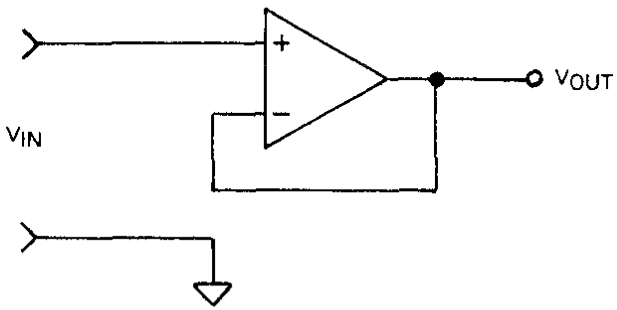
\includegraphics{figuras/instrumental/617volts.png}
        \caption{Tensión}
        %\label{fig:posicionno}
    \end{subfigure}
    \begin{subfigure}[b]{\textwidth}
    \centering
        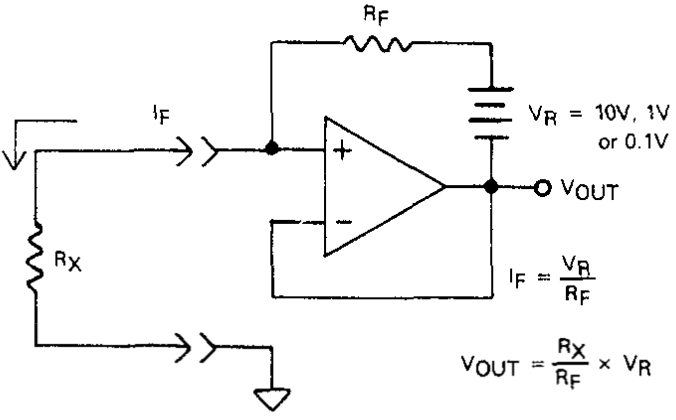
\includegraphics{figuras/instrumental/617ohms.png}
        \caption{Resistencia}
        %\label{fig:posicionno}
    \end{subfigure}
    \begin{subfigure}[b]{\textwidth}
    \centering
        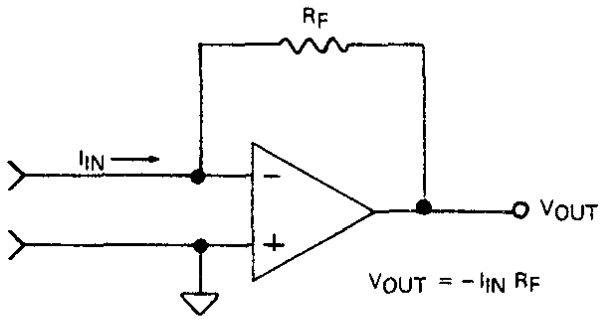
\includegraphics{figuras/instrumental/617amps.png}
        \caption{Corriente}
        %\label{fig:posicionno}
    \end{subfigure}
    \begin{subfigure}[b]{\textwidth}
    \centering
        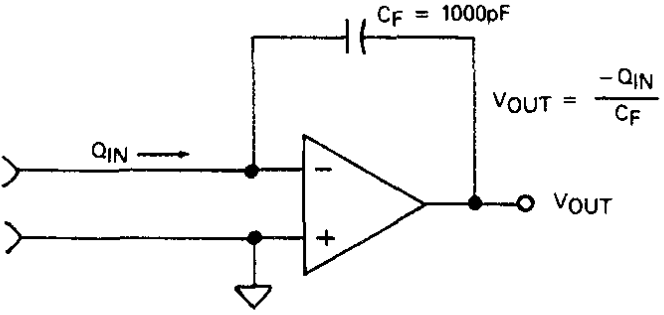
\includegraphics{figuras/instrumental/617coulombs.png}
        \caption{Carga}
        %\label{fig:posicionno}
    \end{subfigure}
    \caption{Configuraciones de medición del electrómetro.
    Reproducido de~\cite{keithley_instruments_inc._keithley_1984}.}
    \label{fig:keithley617}
\end{figure}
Introduciendo elementos de realimentación en el circuito de entrada,
se miden corrientes, resistencias y tensiones 
(\figref{fig:keithley617}).
La alta ganancia del amplificador mantiene la terminal de entrada a
\SI{0}{\volt}, 
evitando cargar el circuito bajo prueba.
\subsubsection{Medición con guarda}
Al medir una fuente de tensión de muy alta impedancia,
cualquier flujo de corriente hacia el instrumento de medición
provoca una caída de tensión considerable.
Debido a la impedancia de entrada del electrómetro,
fluye muy poca corriente a través de sus terminales.
Sin embargo, hay otra corriente que fluye en los cables debido a la resistencia
finita de su aislación (\figref{fig:unguarded}).
\fig{unguarded}{figuras/instrumental/unguarded.png}
{Efecto de las pérdidas de los cables en mediciones de tensión.
    Reproducido de~\cite{keithley_instruments_inc._keithley_1984}.}

Para evitar estas corrientes de pérdida,
se utiliza un conductor de guarda (\figref{fig:guarded})
rodeando al cable de señal.
El electrómetro lo mantiene a una tensión muy cercana a la de la señal.
Esto minimiza la tensión a través del aislante del cable,
reduciendo las pérdidas en el mismo.
Al mismo tiempo, la guarda reduce la capacidad efectiva del cable
al minimizar la diferencia de potencial que aparece entre sus terminales
\cite{rich_shielding_1983}.
\fig{guarded}{figuras/instrumental/guarded.png}
{Medición con guarda para minimizar pérdidas en los cables.
    Reproducido de~\cite{keithley_instruments_inc._keithley_1984}.}
\subsection{Fuente de corriente Keithley 220}
Una fuente de corriente es un instrumento utilizado para forzar corrientes a
través de impedancias grandes,
como la del aislante de gate de un MOS.
Esto requiere una impedancia de salida muy alta para minimizar las pérdidas de
corriente dentro del instrumento.
Al igual que con el electrómetro,
se busca minimizar las corrientes de fuga en el cable de salida.
Para esto se utiliza una guarda al mismo potencial que el cable de señal,
pero forzada desde una fuente de baja impedancia (\figref{fig:220guard}).
\begin{figure}[H]
    \begin{subfigure}[b]{\textwidth}
    \centering
        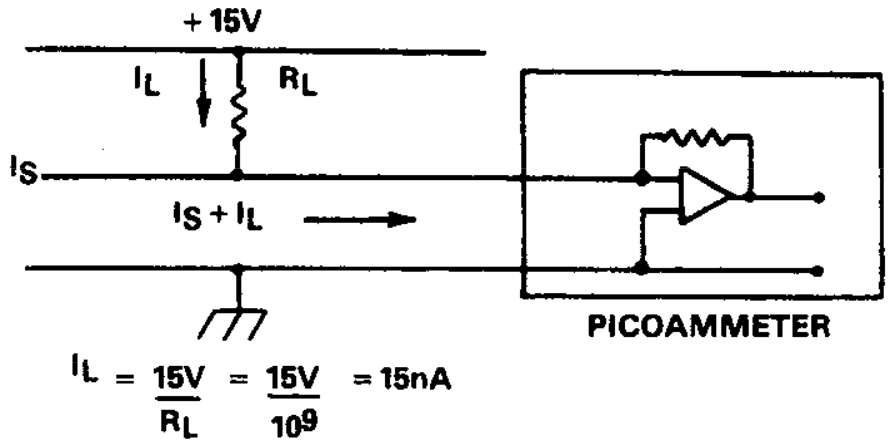
\includegraphics{figuras/instrumental/220unguarded.png}
        \caption{Sin guarda.}
        %\label{fig:posicionno}
    \end{subfigure}
    \begin{subfigure}[b]{\textwidth}
    \centering
        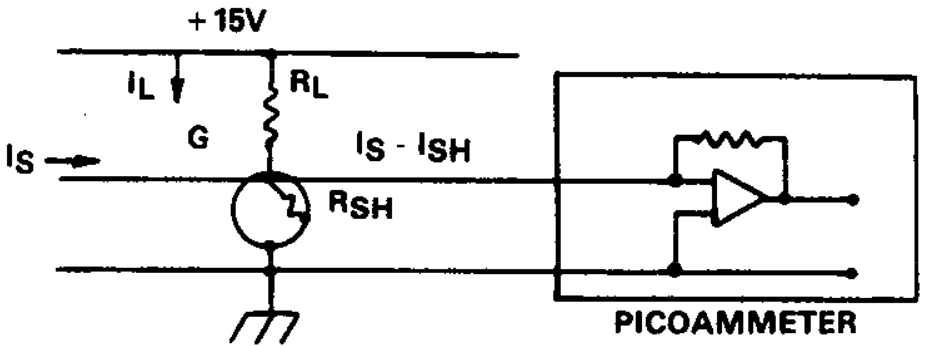
\includegraphics{figuras/instrumental/220guarded.png}
        \caption{Con guarda.}
        %\label{fig:posicionno}
    \end{subfigure}
        \caption{Efecto de las pérdidas al inyectar corriente.
        Rodeando la señal con una guarda, las corrientes de pérdida fluyen en
        la guarda y no afectan la medición.
    Reproducido de~\cite{keithley_instruments_inc._keithley_1984}.}
    \label{fig:220guard}
\end{figure}

\section{Irradiador $\beta$-$\gamma$}
Para realizar ensayos con radiación,
construímos un aparato que nos permite exponer dispositivos a rayos $\beta$ y
$\gamma$ de manera segura para el operario y controlando la dosis con precisión.
Este aparato consiste en un tubo de plomo con una capa de PVC en su pared
interior (\figref{fig:corteirradiador}).
\fig{corteirradiador}{figuras/poster/corte.pdf}{Corte del irradiador.}

Todas las superficies donde puede impactar una partícula $\beta$ tienen una
capa de plástico,
para frenar la partícula con la menor producción posible de
radiación X de frenado.

En un extremo de la cavidad se encuentra una pastilla de \Strontium 
(\figref{fig:fuente})
\fig{fuente}{figuras/poster/fuente.pdf}{Corte de la fuente $\beta$.}
colocada en una mochila de plástico unida a un bloque de plomo giratorio
(\figref{fig:piezagiratoria}).
\fig{piezagiratoria}{figuras/poster/piezagiratoria.png}
{Detalle de la pieza giratoria donde se coloca la fuente $\beta$.}
En una orientación de este bloque,
el mismo se interpone entre la fuente radioactiva y el interior de la cavidad.
Esto permite abrir la cavidad para manipular sus contenidos con seguridad
(\figref{fig:posicionno}).
En la posición de irradiar, la fuente emite partículas $\beta$ hacia el interior
(\figref{fig:posicionsi}).

Gracias al trabajo de Laboratorio 6 y 7 de Javier Badía,
el movimiento de la fuente está motorizado.
Esto permite girar la fuente con un interruptor de manera fácil, rápida y repetible.
\begin{figure}[H]
    \centering
    \begin{subfigure}[b]{.45\textwidth}
        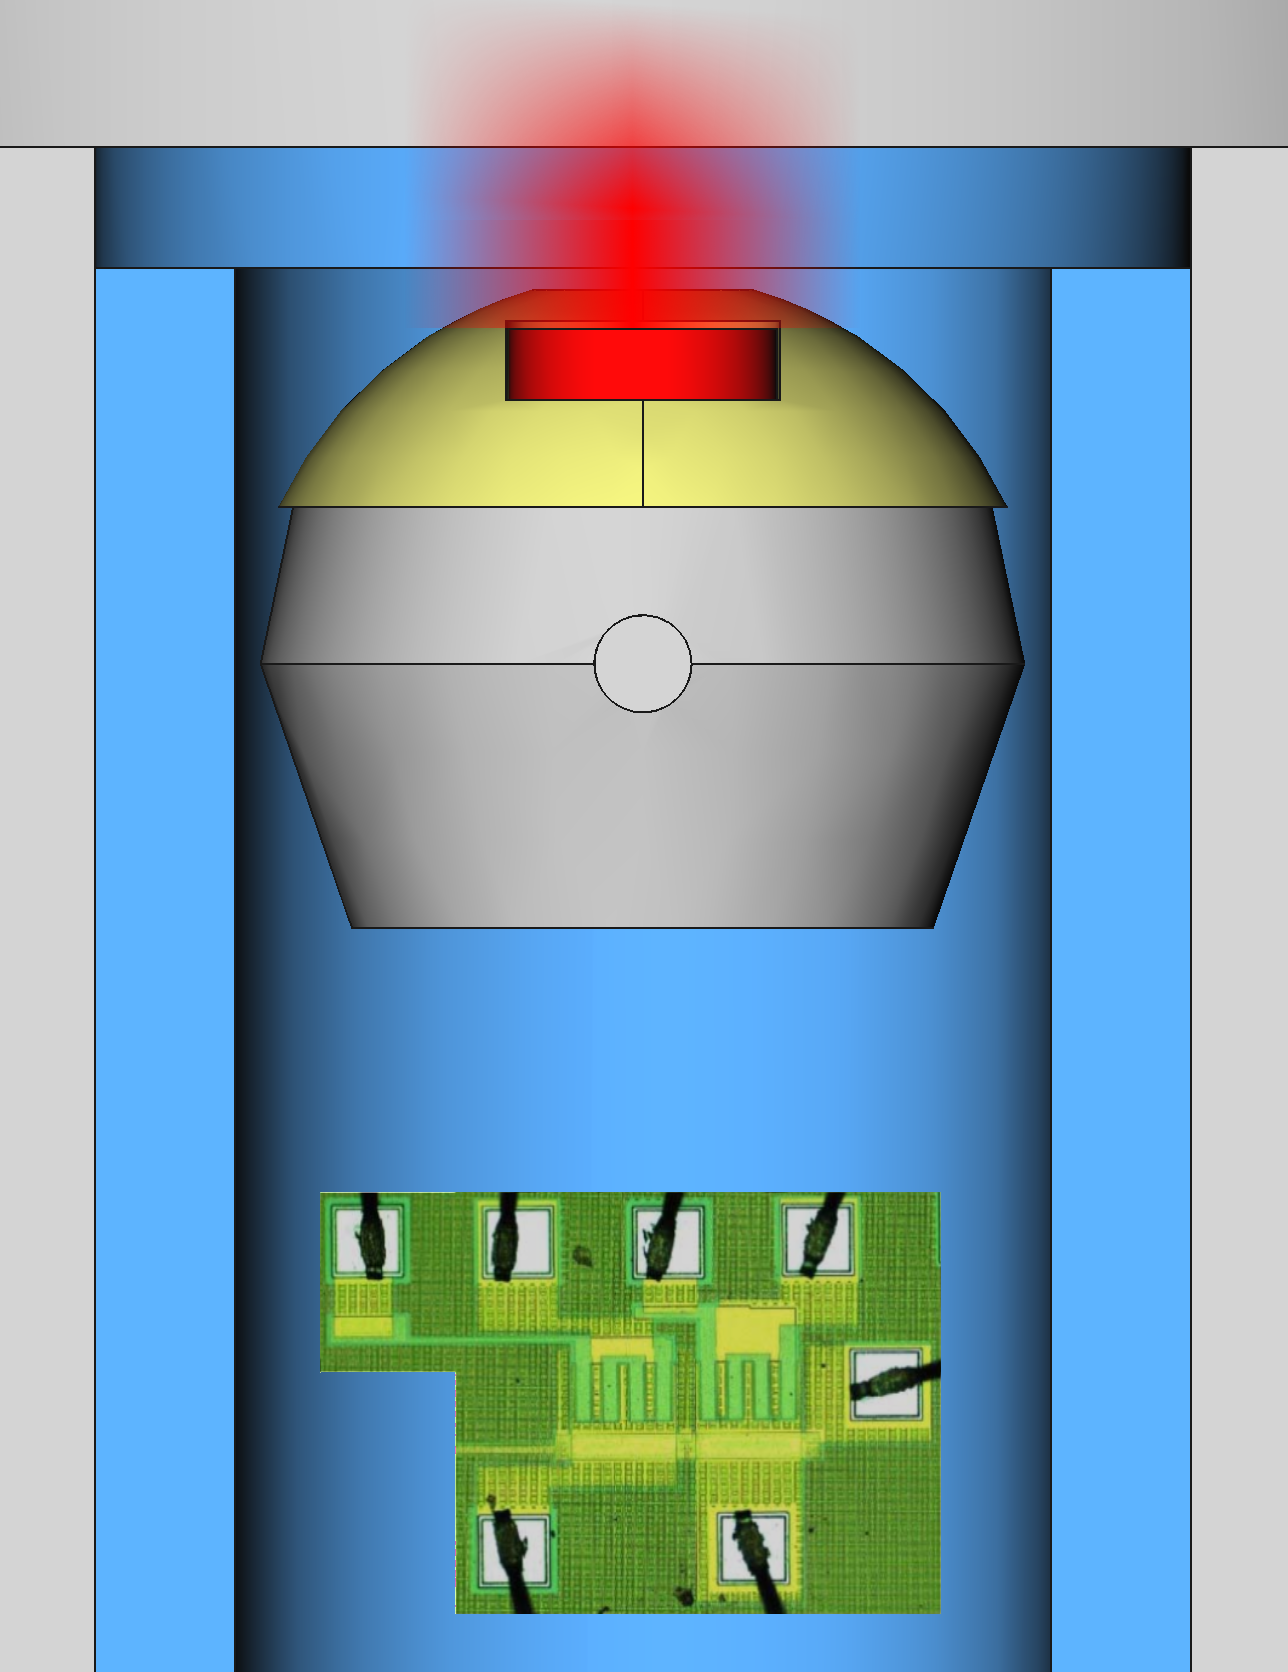
\includegraphics{figuras/poster/posicion_no.png}
        \caption{Posición segura.}
        \label{fig:posicionno}
    \end{subfigure}
    \hspace{5mm}
    \begin{subfigure}[b]{.45\textwidth}
        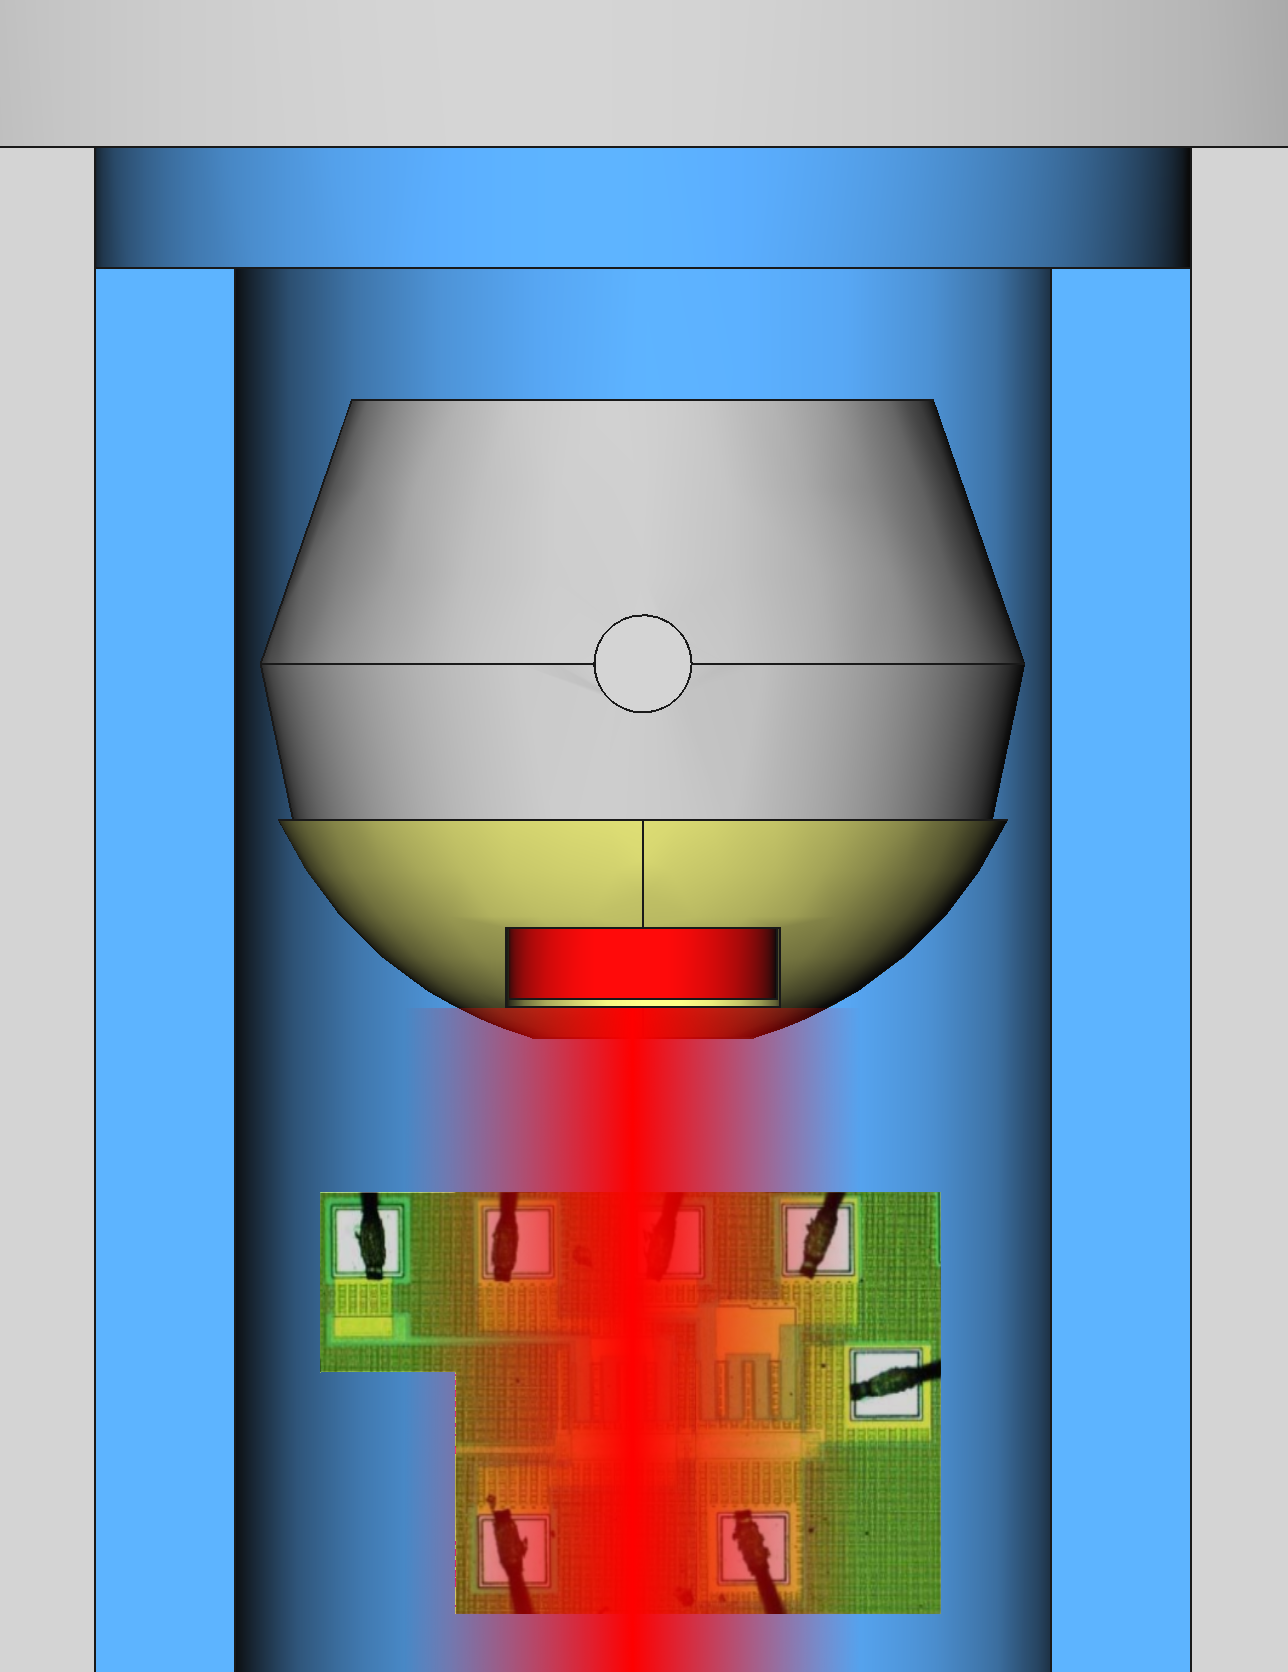
\includegraphics{figuras/poster/posicion_si.png}
        \caption{Posición para irradiar.}
        \label{fig:posicionsi}
    \end{subfigure}
    \caption{Posiciones de la pieza giratoria.}
    \label{fig:posicionespieza}
\end{figure}
\subsection{Construcción}
\subsubsection{Paredes}
Cubrimos ambos extremos de la cavidad con discos de acrílico
de \SI{10}{\milli\meter} de espesor y \SI{90}{\milli\meter} de diámetro.

Para los laterales consideramos moldear tubos de parafina o acrílico
debido a la dificultad de conseguir tubos de PVC con paredes de
\SI{10}{\milli\meter}.
Finalmente optamos por usar un tubo interior y uno exterior de PVC,
y rellenar el espacio intermedio con acrílico.
\subsubsection{Pieza giratoria}
La pieza giratoria está hecha de plomo fundido y luego mecanizado
(\figref{fig:construccion_mariposa}).
\fig{construccion_mariposa}{figuras/irradiador/construccion_mariposa.pdf}
{Pasos para la fabricación de la pieza giratoria de plomo.
El torneado requiere un lugar de donde agarrar a la pieza,
que luego cortamos.}
Para la fundición recurrimos a Abraham Murillo en la 
Escuela Técnica Nº 33 Fundicion Maestranza del Plumerillo. 
Allí tornearon una forma de madera con las dimensiones aproximadas de la pieza final.
La hicimos un poco más grande que las dimensiones finales tomando en cuenta
\begin{itemize}
    \item la contracción del plomo al enfriarse, y
    \item el margen de material extra necesario para tornear.
\end{itemize}
Rodeamos esta forma con tierra apisonada para crear un molde.
El mismo cuenta con un tubo para verter el metal fundido 
y un agujero para ventear gases
(\figref{fig:moldeplomo}).
\fig{moldeplomo}{figuras/irradiador/molde_plomo.pdf}
{Corte del molde usado para fundir la pieza giratoria de plomo.
Está hecho de tierra apisonada alrededor de una forma de madera.
Vertimos el plomo fundido por el tubo de la derecha.
El agujero superior sirve para ventear gases.}
La pieza que sale de este proceso tiene una superficie rugosa
debido a los granos de la tierra usada para el molde.
Para darle una terminación lisa y las dimensiones exactas que necesitamos,
recurrimos a Eriel Fernandez del taller mecánico de FIUBA.
La idea original era darle forma esférica,
pero descartamos esta idea debido a la dificultad
de tornear una esfera en un torno manual.
En cambio, optamos por una forma fácil de tornear
pero que obture lo más posible la cavidad del irradiador 
y pueda girar dentro de la misma
(\figref{fig:torneo_simple}).
\fig{torneo_simple}{figuras/irradiador/torneo_simple.pdf}
{Elegimos una forma simple de tornear que obture lo más posible 
la cavidad del irradiador y pueda girar en su interior.
Para eso nos aseguramos que las esquinas no se salgan de un círculo
con el diámetro interior de la cavidad.}
Las dimensiones finales están en la \figref{fig:torneo}.
La blandez del plomo demandó un torneado cuidadoso a bajas revoluciones.
\fig{torneo}{figuras/irradiador/torneo.pdf}
{Corte lateral de la pieza giratoria de plomo luego del torneado
(dimensiones en mm).}
\subsubsection{Mochila de la fuente}
La fuente va colocada en una pieza de plástico.
Si bien la fuente cuenta con un agujero roscado,
fijarla con un tornillo requiriría manipularla de cerca,
exponiendo las manos a radiación durante cierto tiempo.
Por eso decidimos montarla en un bolsillo donde se puede 
rápidamente dejar caer la fuente,
minimizando la exposición del que realice la tarea.

Quisimos asegurarnos que el plástico frene todos los electrones antes de llegar a
la pieza de plomo. 
Para eso le dimos una forma redonda que cubra lo más posible al plomo,
con la restricción de que pueda girar en la cavidad.

Debido a la dificultad de moldear esta forma (redonda y con una cavidad)
en resina, recurrimos a Iván G. Pollitzer y el 
Laboratorio Abierto de Electrónica.
Iván nos guió en el diseño de una pieza impresa en 3D en ABS.
Esta pieza consiste en dos partes impresas por separado
(\figref{fig:blender}),
\fig{blender}{figuras/irradiador/blender_small.png}
{Las dos partes que imprimimos en 3D en ABS y pegamos para formar la montura de
    la fuente.
Entre las dos partes queda un bolsillo donde se coloca la fuente.}
que luego rellenamos de acrílico y unimos.

Unimos la mochila de plástico a la pieza de plomo usando tornillos sin cabeza,
agujereando y roscando ambas piezas.
\subsection{Cálculos de protección}
\subsubsection{Frenado $\beta$}
Usamos PVC para el frenado de electrones, porque está disponible en tubos
del tamaño requerido.
Tiene baja eficiencia radiativa y el rango de nuestros electrones más
energéticos en PVC es inferior a \SI{1}{\centi\meter}.
Por las mismas razones construimos las tapas del cilindro con discos de
acrílico de \SI{1}{\centi\meter} de espesor.
La mochila donde montamos la fuente consiste de plástico ABS 
extruído en una impresora 3D en el LABi.
Esto requirió separar el modelo inicial en dos partes que fueron pegadas y
terminadas con herramientas manuales.
%
\subsubsection{Cálculos de radiación de frenado}
Las partículas $\beta$ de la fuente empiezan a frenarse en el plástico,
donde producen radiación X de frenado.
Estimamos su magnitud partiendo del espectro de energía de los
electrones emitidos por la fuente.
Dado que está en equilibrio secular 
(misma actividad de \Strontium y de \Yttrium),
sumamos sus espectros provenientes de 
Radiological Toolbox\cite{eckerman2006radiological}
y normalizamos a la actividad nominal de la fuente, \SI{100}{\milli\curie}
(\figref{fig:actividadsr90}).
\fig{actividadsr90}{figuras/irradiador/actividad.pdf}
{Espectro de electrones provenientes de una fuente de
\Strontium con actividad \SI{100}{\milli\curie}\cite{eckerman_icrp_2007}.}
Luego calculamos el espectro de bremsstrahlung integrando la \equref{eq:kramers}
(\figref{fig:espectrox}).
\fig{espectrox}{figuras/irradiador/espectrox.pdf}
{Espectro de bremsstrahlung calculado en la cara exterior del PVC.}
%
\subsubsection{Atenuación de rayos X en el plomo}
Aplicamos la \equref{eq:absorcionx} 
usando tasas de absorción en plomo tabuladas por NIST\cite{xraycoef},
resultando en el espectro atenuado de la \figref{fig:xatenuado}
\fig{xatenuado}{figuras/irradiador/xatenuado.pdf}
{Espectro de rayos X calculado en la cara exterior del irradiador.}
% TODO: tasa de dosis final según distancia, comparar con mediciones
%
%
\subsubsection{Cálculos Monte-Carlo de fuente de \Strontium}
La fuente de \Strontium  emite electrones con un espectro amplio de
energías (\figref{fig:actividadsr90}).
Este consiste en la suma del espectro de emisión de \Strontium
y el de \Yttrium.
Simulamos un haz de electrones con este espectro incidiendo normalmente sobre
tejido blando, registrando la energía que depositan en función de la
profundidad (\figref{fig:deposicionsr90}).
\fig{deposicionsr90}{figuras/montecarlo/deposicion_sr90.pdf}
{Energía depositada en tejido blando en función de la distancia,
promediando entre electrones provenientes de una fuente de \Strontium.}
Así ajustamos una potencia de frenado de masa promedio $S/\rho$ (\figref{fig:stoppingsr90})
\fig{stoppingsr90}{figuras/montecarlo/stopping_sr90.pdf}
{Potencia de frenado promedio del tejido blando para electrones provenientes de
una fuente de \Strontium.
La cruz marca que a una profundidad de \SI{0.35}{\milli\meter} la tasa de dosis 
coincide con la tabulada en \cite{delacroix_radionuclide_2002}.}
que permite calcular tasa de dosis superficial mediante
\begin{align*}
    \dot D &= \frac{AS/\rho}{4\pi r^2}
\end{align*}
con $A=\SI{100}{\milli\curie}$ la actividad de la fuente.
La tasa de dosis calculada de este modo es comparable con la tabulada en
\cite{delacroix_radionuclide_2002} si se promedia hasta una profundidad de
\SI{.35}{\milli\meter}.
Esto sirve como verificación de que nuestras simulaciones Monte-Carlo producen
valores compatibles con los que se encuentran en la literatura.
\subsubsection{Cálculos Monte-Carlo del irradiador}
Buscamos una cota superior de la tasa de dosis fuera del irradiador.
Esto brinda la mayor confianza en que su operación no es peligrosa.
Ya que el espesor del plomo es de varias longitudes características de
atenuación ($1/\mu$),
sólo pasa una fracción muy pequeña de la radiación inicial.
Por lo tanto, hay que simular la emisión de 
muchos electrones de la fuente de \Strontium
para que llegue una cantidad apreciable a la cara exterior.
Así podemos estimar de forma precisa la tasa de dosis.

Una solución posible es usar reducción de la
varianza\cite{dressel_geometrical_2003}.
Esta es una técnica para cálculos Monte Carlo que introduce un sesgo en la
evolución de la partícula.
Por ejemplo, podemos aumentar la probabilidad de que una partícula atraviese
el plomo sin interactuar, en vez de scatterear.
Llevando la cuenta de cuan improbable es la historia de la partícula,
le damos un peso menor en la estadística final.
Esto concentra la simulación en darnos muchos eventos que nos interesan
(lo cual reduce la varianza de la estimación),
minimizando la capacidad de procesamiento necesaria.

Dada la dificultad de implementar reducción de la varianza en Geant4,
optamos por acelerar el cálculo simplificando la geometría.
Simulamos un irradiador con simetría esférica,
que consiste en un cascarón de \SI{10}{\milli\meter} de acrílico rodeado por
\SI{36}{\milli\meter} de plomo (\figref{fig:corte_esferico}). 
\fig{corte_esferico}{figuras/irradiador/corte_esfera.png}
{Corte de la geometría simplificada que se usó para simular el irradiador en
Geant4.}
Toda partícula en el irradiador tiene que atravesar al menos ese espesor de
acrílico y plomo.
Por lo tanto, la dosis real va a ser aún menor a la simulada.
Dada la simetría del problema, no tenemos en cuenta la distribución en
$\theta$ y $\phi$ sino que promediamos sobre ambas variables.
Esto reduce enormemente el número de eventos necesarios para una buena
estimación de la tasa de dosis.
El resultado se ve en la \figref{fig:dosis_irradiador}.
\fig{dosis_irradiador}{figuras/montecarlo/dosis_irradiador.pdf}
{Perfil de deposición de energía en la simulación Monte-Carlo del irradiador.}
La dosis en la cara exterior del irradiador es
de \SI{20.3}{\milli\sievert\per\year}.
Este valor es aceptable si se tiene en cuenta que,
en condiciones reales, se toca el irradiador durante intervalos muy cortos
y el resto del tiempo se está a distancias mucho mayores.

\part{Diseño, fabricación y caracterización de dosímetros MOS no
convencionales}
\section{Dosímetro Active Pixel Sensor}
\fig{aps}{esquematicos/aps.pdf}{Esquemático del dosímetro APS}
El dosímetro APS tiene una estructura similar a 
un pixel del sensor de imagen en una cámara digital. 
Requiere alimentación durante la irradiación,
pero puede operar con tensiones pequeñas
como las que provee una batería.
Asimismo, tiene la ventaja de poder resetearse rápidamente.
Esto permite tomar mediciones con gran resolución temporal.

Esta parte del trabajo comienza con la teoría del dosímetro.
Luego cubre cómo realizamos el diseño y lo optimizamos.
Por último, presenta las mediciones del sensor fabricado 
y las conclusiones que siguen de ellas.
%
\subsection{Principio de funcionamiento}
%
Su principio de funcionamiento es medir 
la carga generada por radiación 
en la zona desierta de una juntura p-n.
El cátodo de la juntura está aislado eléctricamente 
para acumular la carga generada sin que se fugue
(D1 en \figref{fig:aps}).
Antes de cada medición, se reinicia el circuito llevando dicho cátodo a
V$_{\text{DD}}$ prendiendo brevemente el transistor de reset M1.
La radiación que incide en la zona desierta de D1 interactúa con la red de
silicio, depositando energía a través de distintos procesos como scattering e
ionización (ver sección~\ref{sec:radiacion}).
Los fotones y electrones secundarios resultantes producen pares electrón-hueco,
que son arrastrados en direcciones opuestas por el campo eléctrico
que existe normalmente en la zona desierta.
Los electrones se acumulan en el cátodo,
descargándolo gradualmente hacia \SI{0}{\volt}.
Luego de irradiar,
se mide su tensión a través de un par de seguidores M2 y M3.
Los mismos forman un circuito que replica la tensión de entrada a la salida,
pero desplazada un valor fijo.
Su propósito es evitar que la medición de tensión modifique la carga en el nodo y
afecte al valor medido.
\subsection{Trabajos previos}
Turchetta\cite{turchetta_monolithic_2001} describe un APS para rayos X
construído en un proceso CMOS estándar de \SI{0.6}{\micro\meter}. 
Construye una grilla de píxeles para uso en tracking de partículas.
Expone el sensor a rayos X provenientes de \isotope{Fe}{55},
y a piones de \SI{15}{\giga\electronvolt}.
Expresa la sensibilidad en términos de Volts por electrón generado por
radiación. Esta figura llega a \SI{15}{\micro\volt} por electrón,
con un ruido RMS equivalente a 15 electrones.
Una innovación es el uso de un layout que permite que casi toda la superficie
del wafer sea sensible.

Matis\cite{matis_charged_2003} también construye un array de APS,
en un proceso estándar de \SI{0.25}{\micro\meter}.
Analiza distintas formas de procesar la señal,
sumando la salida de varios píxeles para colectar toda la carga generada por
una partícula incidente.
Irradia el sensor con rayos X provenientes de \isotope{Fe}{55},
y protones de \SI{55}{\mega\electronvolt}.
\subsection{Proceso de fabricación}
Si bien la fabricación viene luego del diseño,
todo el diseño está condicionado por 
las características del proceso de fabricación.
En específico,
\begin{itemize}
    \item qué tensiones soporta,
    \item qué dispositivos provee, y
    \item qué características eléctricas tienen esos dispositivos
        (tensiones umbral, capacidades parásitas, corrientes de pérdida, etc).
\end{itemize}

Fabricamos tanto el FG como el APS en el proceso XC06 de la foundry X-FAB
\cite{x-fab_0.6_2008}.
El mismo tiene una escala (longitud característica) de \SI{0.6}{\micro\meter} y está diseñado para
tensiones de hasta \SI{5}{\volt}.
En su versión estándar, 
cuenta con 1 capa de polisilicio y 2 de metalización.
Existen variantes del proceso que utilizan máscaras adicionales para,
por ejemplo, abrir ventanas para formar regiones fotosensibles.
\subsection{Reset}
Cargamos el nodo flotante a través del drain de un MOSFET de canal P,
con el source conectado a \vdd.
Durante la irradiación llevamos su gate a \vdd, apagándolo.
Para resetear 
llevamos su gate a tierra.
Esto lo coloca en saturación,
cargando la juntura a corriente constante 
y aumentando $V_D$ linealmente hasta $V_t$.
Entonces entra en triodo y va reduciendo la corriente,
cargando asintóticamente hasta \vdd.
Esto permite llevarlo a $V_{dd}$,
mientras que una llave de tipo N sólo llegaría hasta $V_{dd}-V_{tn}$ antes de
apagarse.

El transistor de reset es de área mínima,
para que aporte la menor capacidad parásita posible al nodo flotante.
Esto, como se verá más adelante, maximiza la sensibilidad del sensor.
\subsection{Respuesta a partículas}
Cada partícula incidente deposita una energía promedio que depende de su energía
cinética inicial\cite{berger_response_1969} (ver sección~\ref{montecarloaps}).
Una fracción $E$ de esta energía se usa en la creación de pares electrón-hueco,
generando carga 
\begin{align*}
    Q &= \frac{qE}{E_i}
\end{align*}
con $q$ la carga del electrón y $E_i$ la energía de creación de pares,
\SI{3.62}{\electronvolt} en Si.
Esta carga aparece con signo negativo en el cátodo, descargándolo.
Su cambio de tensión
\begin{align*}
    \Delta V &= \frac{\Delta Q}{C}
\end{align*}
depende de la capacidad total $C$ del nodo.
La misma tiene contribuciones de
\begin{itemize}
    \item juntura de D1,
    \item juntura Drain-Body de M1,
    \item Gate de M2, y
    \item conductores cercanos al nodo.
\end{itemize}
Estas capacidades pueden estimarse a partir de las especificaciones del 
proceso de fabricación,
que indican capacidad por unidad de área y por unidad de perímetro.
Para eso usamos herramientas de EDA (electronic design automation)
que realizan esta estimación automáticamente a partir de la geometría del
diseño (ver sección~\ref{section:diseno_aps}).
\subsection{Cálculos Monte-Carlo}
\label{montecarloaps}
El dosímetro APS detecta energía depositada 
en una región específica de un circuito integrado.
A fines de simularlo, 
simplificamos la geometría del die en tres regiones:
una superficie de SiO$_2$, un sustrato de Si 
y una zona sensible también de Si (\figref{fig:corteaps}).
\fig{corteaps}{figuras/aps/corte.pdf}
{Corte de la geometría usada para simular el APS en Geant4 (no a escala).}
Las dimensiones se extrajeron del diseño del APS 
y de las especificaciones del proceso de fabricación del chip.

Dado que el uso principal de Geant4 es en física de altas energías,
su configuración por defecto no permite simular electrones secundarios por
debajo de \SI{250}{\electronvolt}.
% DETAIL rango a 250eV ~ nm, qué me importa?
Para obtener precisión a escalas de distancia más chicas,
empleamos una lista de procesos de interacción 
compilada para simulaciones en microelectrónica \cite{Raine201497}.
La misma simula con fidelidad electrones hasta \SI{16.7}{\electronvolt},
cuyo rango en Si es del orden de \SI{0.1}{\nano\meter}.

Los resultados se encuentran en la \figref{fig:energia1electron}.
% FIXME falta este gráfico usando
% ../tesis/figuras/aps/deposicion1electron001.pdf y demás
\fig{energia1electron}{figuras/aps/deposicion1electron_todos.pdf}
{Distribución de probabilidad simulada en Geant4 
    para la energía depositada en el sensor (eje X).
Cada gráfico corresponde a una dada energía cinética de la partícula incidente.
La energía promedio depositada está en la \figref{fig:energiadepositadaaps}.}
Se ve que los electrones menos energéticos tienden a frenarse por completo en
el detector, depositando toda su energía.
Los más energéticos, en cambio, depositan una fracción variable de su energía
total.
La energía depositada promedio se encuentra en la
\figref{fig:energiadepositadaaps}.
\fig{energiadepositadaaps}{figuras/poster/aps_respuesta.pdf}
{Respuesta promedio a un electrón incidente,
en función de su energía inicial.
Se ve que los electrones menos energéticos se frenan completamente en el
detector.
Las cruces son el resultado de simulación con Geant4,
mientras que la línea es un cálculo manual 
con los datos tabulados por NIST en ESTAR\cite{berger_estar_????}.}
Se ve que para el rango de energías de interés,
cada partícula incidente produce un cambio de decenas de mV.
\subsection{Fuentes de ruido}
El APS se maneja con corrientes y variaciones de carga y tensión muy
pequeñas.
Por eso es crítico conocer los procesos que introducen ruido, 
y su magnitud.
Este ruido se combina con la señal proveniente de la radiación
y determina la resolución del dosímetro: 
la dosis mínima que es posible resolver por encima del ruido.
% TODO: citar 
% Taylor, John Robert (1999). An Introduction to Error Analysis:
% The Study of Uncertainties in Physical Measurements. University Science
% Books. pp. 128–129. ISBN 0-935702-75-X.
\subsubsection{Corriente de fuga de juntura p-n}
Al polarizar una juntura p-n en inversa, fluye una corriente de
pérdida\cite{sze_physics_2007} con un valor de DC dado por
\begin{align*}
    I&=I_s(e^{\frac{qV}{\eta kT}}-1)
\end{align*}
con $V<0$ la tensión aplicada y $I_s$ y $\eta$ parámetros de fabricación de la
juntura.
El valor instantáneo de $I$ fluctúa debido a la naturaleza discreta de los portadores que
atraviesan la barrera de energía de la juntura.
Esta fluctuación se denomina ruido \emph{shot}, una clase de ruido blanco:
su densidad espectral de potencia,
\begin{align*}
    i^2(f) &= 2q|I|,
\end{align*}
no varía con la frecuencia (hasta frecuencias muy altas).
\subsubsection{Fluctuaciones durante reset}
Durante el reset, se carga la juntura p-n hasta $V_{dd}$ a través de M1.
Cerca de la tensión final, M1 entra en modo triodo.
En esta condición de operación, el canal actúa como una resistencia.
Esto significa que produce ruido de Johnson\cite{baker_cmos_2010}.
Al cargar la capacidad de juntura $C$, 
este ruido produce una varianza en la tensión final dada por
\begin{align*}
    \overline{v^2} &= \frac{kT}C.
\end{align*}
Evaluando esta fórmula con la capacitancia del APS
% TODO: es la capacidad de 4x4 o 40x40?
se llega a una tensión de ruido RMS de \SI{1.1}{\milli\volt}.

Esta incertidumbre en la tensión luego del reset puede eliminarse usando 
la técnica Correlated Double Sampling\cite{white_characterization_1974}:
se mide tensión antes y después de la exposición a la radiación.
Al tomar la diferencia se elimina el ruido de reset,
presente en ambas por igual.

\subsection{Diseño del circuito}
\label{section:diseno_aps}
La topología del circuito quedó determinada por la elección de construir un
dosímetro APS con un par de seguidores para su medición.
El paso siguiente en el diseño fue elegir los tamaños de los distintos
componentes para optimizar el desempeño del sensor.

Para una carga dada, la tensión sobre un capacitor es inversamente proporcional
a su capacidad.
En el APS la carga es generada por la radiación,
y la tensión es la señal cuya magnitud queremos maximizar.
Para esto minimizamos las capacidades parásitas del cátodo de D1,
usando transistores de área mínima para M1 y M2.
Restringimos el largo de las conexiones del cátodo,
y las mantuvimos alejadas de otros nodos.
Aplicamos software de Mentor de extracción de capacidades parásitas al layout
resultante, y obtuvimos una capacidad total en el cátodo de \SI{3.4}{\femto\farad}.

El tamaño del primer MOS seguidor, M2, 
tiene que ser el tamaño mínimo para no cargar capacitivamente
al nodo que acumula carga.
Esto deja libre las dimensiones del segundo MOS seguidor, M3.
Mientras más grande es, mayor es su capacidad de gate
y por lo tanto más va a cargar a la etapa anterior.
Por otro lado va a tener mayor capacidad de corriente
para manejar la carga capacitiva del pad de salida.

Estimamos un tamaño inicial para M3 fijando un largo arbitrario
y variando el ancho para minimizar una figura de mérito.
La figura que elegimos representa el delay producido por los dos seguidores,
\begin{align}
    \tau &= \tau_1+\tau_2 = g_{m2}C_{g3} + g_{m3}C_{\textnormal{pad}}
    \label{eq:delay_seguidor_aps}
\end{align}
con $g_m=\pderiv{I_D}{V_G}$ la transconductancia de un MOS 
y $C_g$ su capacidad de gate.
Minimizando la ecuación~\ref{eq:delay_seguidor_aps}
para una polarización pre-fijada,
llegamos a un $W$ inicial de \SI{409}{\micro\meter}.

El paso siguiente es hacer un cálculo más preciso 
que incluya todos los detalles del funcionamiento del circuito.
Para esto simulamos con SPICE el tiempo de respuesta a un electrón incidente
en función del ancho de M3 (\figref{fig:falltime}). % FIXME función de qué?
\fig{falltime}{figuras/aps/falltime.pdf}
{Tiempo de respuesta simulado del buffer en función del ancho del MOS del
    segundo seguidor. 
    $W_{\textnormal{ideal}}$ es el $W$ óptimo cálculado a mano de forma
    simplificada.
}
Se ve que hay poca mejora en el tiempo de respuesta 
al aumentar $W$ por encima de nuestro estimado inicial.
Por eso, teniendo en cuenta las limitaciones de área,
elegimos un ancho total de \SI{400}{\micro\meter} repartido entre 8 canales 
(o sea 8 MOS en paralelo, cada uno de \SI{50}{\micro\meter}).

Las dimensiones finales están en la tabla~\ref{fig:areas_aps}.
\begin{table}[h]
    \centering
    \caption{Dimensiones del diseño optimizadas para sensibilidad y tiempo de
    respuesta}
    \begin{tabular}{|c|c|c|c|}
        \hline
        Dispositivo&      W (um)&    L (um)&  Canales\\
        \hline
D1&     4&  4&  1\\
M1&     0.8&    0.6&    1\\
M2&     0.8&    0.6&    1\\
M3&     50& 3&  8\\
        \hline
    \end{tabular}
    \label{fig:areas_aps}
\end{table}

Estas dimensiones se utilizaron tanto para la simulación del circuito en SPICE
como para los cálculos Monte-Carlo.
La combinación de estas dos herramientas nos da una sensibilidad esperada de 
\SI{7.1}{\volt\per\gray}.
El diseño físico final está en la \figref{fig:layoutaps}.
\begin{figure}[p]
    \centering
    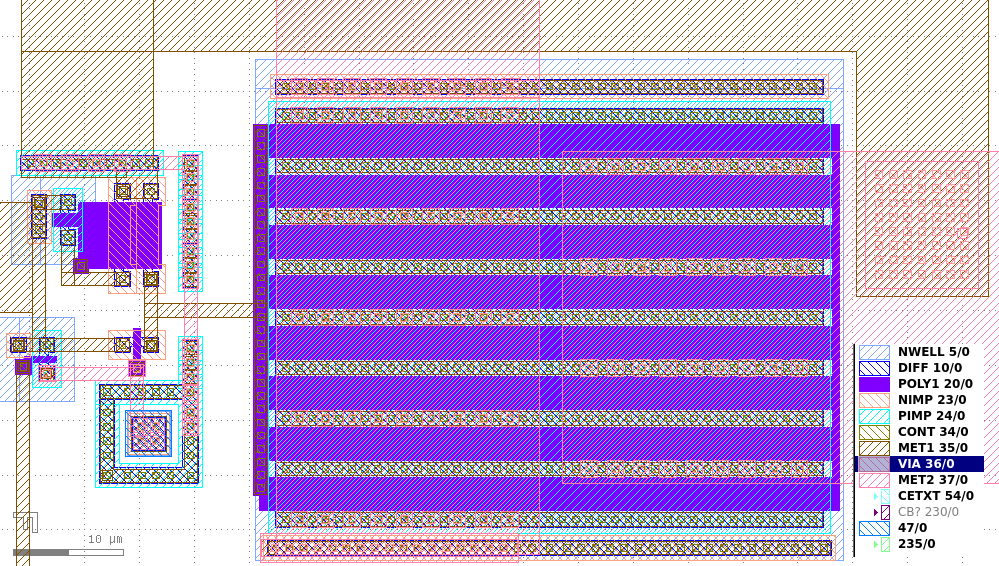
\includegraphics[width=\columnwidth]{figuras/gds/aps/todo.png}
    \caption{Layout del dosímetro APS. 
    El transistor de la derecha es el de salida, del segundo seguidor.
    El resto se ve en más detalle en la \figref{fig:layoutapszoom}.}
    \label{fig:layoutaps}
\end{figure}
\begin{figure}[p]
    \centering
    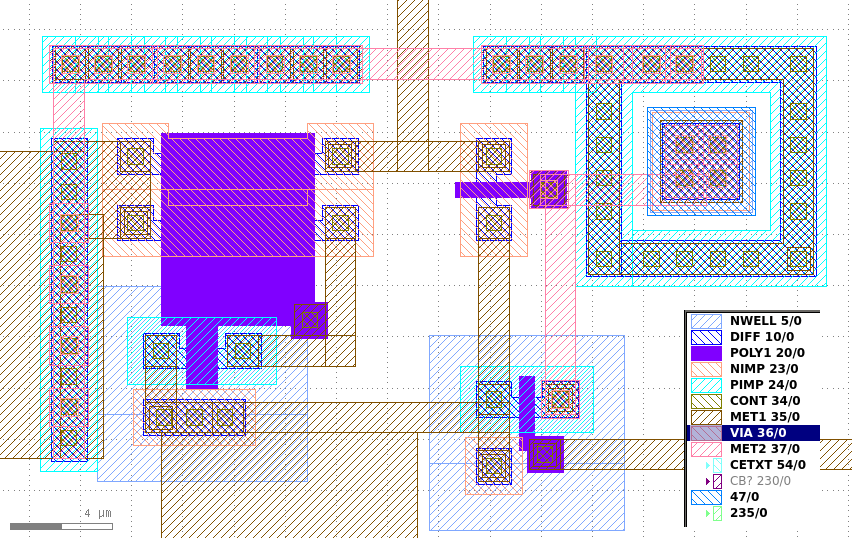
\includegraphics[width=\columnwidth]{figuras/gds/aps/zoom.png}
    \caption{Vista en detalle del layout del APS, excluyendo el transistor de
        salida.
        A la derecha está el diodo, con el cátodo (nwell) en el centro y el
        ánodo (contactos a sustrato) rodeándolo.
        A su izquierda está el primer MOSFET seguidor y abajo el MOSFET de
        reset.
        Los transistores de la izquierda polarizan al primer seguidor.
    El transistor de reset está conectado a un pad (no visible) a través del
    circuito de protección de la \figref{fig:proteccion5v}.}
    \label{fig:layoutapszoom}
\end{figure}
\fig{proteccion5v}{figuras/aps/proteccion.pdf}
{Circuito de protección para la entrada de reset.
Los diodos sólo conducen si la tensión del pad excede \SI{5}{\volt} o
baja de \SI{0}{\volt}.
Cuando llega un pulso de alta tensión
(por ejemplo debido a una descarga electrostática)
los diodos limitan la tensión que llega al circuito.
Esto evita que se polaricen en directa las junturas drain-body y source-body,
previniendo una falla por latchup (sección~\ref{latchup}).
También evita la ruptura de los óxidos de compuerta de MOS.}
\subsection{Medición}
Tomamos dos dies y los bondeamos a placas adaptadoras de TSSOP28,
un tipo de empaquetado de circuitos integrados de montaje superficial
(figuras~\ref{fig:bondeados1}, \ref{fig:bondeados2} y~\ref{fig:pinout}).
\fig{bondeados1}{figuras/aps/bondeados.jpg}
{Dies bondeados a placa adaptadora SMD.
Los zócalos tienen las patas cortocircuitadas para proteger al die de
descargas electrostáticas durante el transporte y almacenamiento.}
\figp{bondeados2}{figuras/aps/die.jpg}
{Detalle del die fabricado con los dosímetros APS y FG 
(arriba en la columna central)
y otros circuitos.}
\figp{pinout}{figuras/aps/pinout1.pdf}
{Layout del die entero con numeración de los pads bondeados}
\subsubsection{Descarga en oscuridad}
Primero medimos la respuesta del sensor sin luz ni radiación
(figuras~\ref{fig:oscuridad4} y~\ref{fig:oscuridad40}).
\fig{oscuridad4}{figuras/aps/oscuridad4.pdf}
{Curva de descarga en oscuridad del APS de 4x\SI{4}{\micro\meter}.
Resulta de resetear el APS y medir su tensión de salida en oscuridad.}
\fig{oscuridad40}{figuras/aps/oscuridad40.pdf}
{Curva de descarga en oscuridad del APS de 40x\SI{40}{\micro\meter}.
Resulta de resetear el APS y medir su tensión de salida en oscuridad.}
Esto nos muestra la descarga del diodo debido a la corriente de fuga en
inversa.

Se ve en ambas figuras la misma curva 
con escalas distintas de tiempo y de tensión.
Esta variación proviene tanto de las áreas distintas de los dos sensores
como de las variaciones aleatorias entre los MOS seguidores (mismatch).
Cada transistor del die tiene pequeñas variaciones debido a imperfecciones en
la litografía y variaciones aleatorias de dopaje.
Estas variaciones no son tan notables en dispositivos grandes debido a que
se cancelan al promediarse sobre mucha área.

Ya que los seguidores usan varios transistores de área mínima,
son particularmente sensibles a variaciones del proceso:
el mismo error absoluto en las dimensiones del canal produce un mayor error relativo.

% Descarga debería ser lineal
% https://books.google.com.ar/books?id=6Rg7AAAAQBAJ&lpg=PA289&ots=yO1HPv_N4E&dq=reverse%20biased%20diode%20%22discharge%20curve%22&hl=es&pg=PA290#v=onepage&q=reverse%20biased%20diode%20%22discharge%20curve%22&f=false

La curva de descarga es la solución a una ecuación diferencial
no-lineal:
\begin{align*}
    \frac{\partial Q}{\partial V}\frac{dV}{dt} &= -I(V)
\end{align*}
La forma de la curva proviene de la variación 
tanto de la corriente de fuga $I(V)$ 
como de la capacidad del diodo $\frac{\partial Q}{\partial V}(V)$.
Ambas dependen de la tensión aplicada,
debido a la variación del ancho de la zona desierta.
Al caer la tensión en inversa,
la zona desierta se vuelve más angosta.
Esto reduce su volúmen y por lo tanto 
la tasa de generación térmica de pares electrón-hueco.
Por otra parte,
su capacidad es inversamente proporcional a este ancho.
Ambos fenómenos reducen la tasa de descarga,
como se ve al final de ambas curvas.

Por otro lado, hay factores de segundo orden 
que no contemplamos en el análisis.
Por ejemplo, el transistor de reset apagado
no es un circuito abierto perfecto, 
sino que tiene una corriente de pérdida muy pequeña.
Esta corriente va a tender a cargar el cátodo de D1,
enlenteciendo la descarga.
%
\subsection{Iluminación con LED}
Medimos las curvas de descarga iluminando los dies con un LED,
variando su corriente para lograr distintas intensidades de iluminación
(figuras~\ref{fig:led4} y~\ref{fig:led40}).
\fig{led4}{figuras/aps/descarga_led_4.pdf}
{Curva de descarga iluminando con un LED el APS de 40x\SI{40}{\micro\meter}.
La corriente del LED aumenta de \SI{.1}{\milli\ampere} a la derecha hasta
\SI{10}{\milli\ampere} a la izquierda,
con 6 curvas por década.}
\fig{led40}{figuras/aps/descarga_led_40.pdf}
{Curva de descarga iluminando con un LED el APS de 4x\SI{4}{\micro\meter}.
La corriente del LED aumenta de \SI{.1}{\milli\ampere} a la derecha hasta
\SI{10}{\milli\ampere} a la izquierda,
con 6 curvas por década.}
Esto permite observar la compresión de la curva de descarga 
con el aumento de la radiación incidente.
\subsubsection{Ruido medido}
Establecimos que una medición con este dosímetro consiste en promediar 10
muestras de tensión.
Esto nos permite definir de manera precisa el ruido como la desviación estándar
de ese promedio.
Calculamos esa desviación estándar en base a las curvas medidas (figuras~\ref{fig:ruido4} 
y~\ref{fig:ruido40}).
\fig{ruido4}{figuras/aps/ruido4.pdf}{Ruido a la salida del APS de
    \SI{4x4}{\micro\meter}, calculado tomando diferencias entre muestras y
escalando para que represente el ruido en un promedio de 10 valores.}
\fig{ruido40}{figuras/aps/ruido40.pdf}{Ruido a la salida del APS de
    \SI{40x40}{\micro\meter}, calculado tomando diferencias entre muestras y
escalando para que represente el ruido en un promedio de 10 valores.}
Podemos convertir estos valores de ruido en dosis usando la sensibilidad
calculada.
Así llegamos a una resolución de \SI{2.0}{\milli\gray} y \SI{2.3}{\milli\gray}
para el APS de \SI{4x4}{\micro\meter} y \SI{40x40}{\micro\meter},
    respectivamente.
% TODO ? completar con cálculos de sensibilidad/resolución y mediciones.
%
\subsection{Conclusiones}
Presentamos el concepto básico del dosímetro APS,
con sus peculiaridades de uso y el tipo de mediciones que permite realizar.
Cubrimos su teoría de funcionamiento,
y de ahí explicamos el proceso de diseñar el circuito
para su fabricación.

En los resultados verificamos que el sensor
sigue el comportamiento básico que esperamos,
tanto en ausencia de radiación 
como para distintas intensidades de luz visible.
Asimismo, conseguimos una estimación inicial de la resolución del sensor
en base al ruido medido a la salida.
Así dimos los primeros pasos para implementar un dosímetro APS
en un proceso de fabricación CMOS estándar.

\section{Dosímetro Floating Gate}
Los MOSFET con gate aislado o floating gate se usan comercialmente
en memorias no volátiles (Flash y EEPROM).
Se coloca cierta carga, 
cuyo valor representa uno o más bits de información, en el gate.
Luego se recupera la información midiendo la carga del gate
en base a las curvas IV del MOSFET.

El dosímetro FG se basa en un MOSFET con gate aislado.
Su modo de uso es primero resetearlo, dándole una carga inicial.
Desde el momento de reset, el dosímetro integra 
la dosis total que recibe sin necesidad de alimentación
(mientras no exceda una dosis máxima).
Por lo tanto es idóneo para seguimientos largos,
por ejemplo de un trabajador durante su turno.

Igual que como hicimos para el dosímetro APS,
esta parte del trabajo comienza con la teoría del dosímetro.
Luego cubre cómo realizamos el diseño y lo optimizamos.
Por último, presenta las mediciones del sensor fabricado,
incluyendo los resultados de su irradiación,
y las conclusiones que siguen de ellas.
%
\subsection{Principio de funcionamiento}
El principio de funcionamiento del dosímetro FG 
es que la radiación que incide
en el óxido de compuerta tiende a descargar al FG.
Antes de irradiar,
se coloca carga en el gate mediante una corriente de túnel 
(\figref{fig:cargafg}).
\figp{cargafg}{figuras/fg/esquemainyeccion.pdf}
{ Inyección de carga en el FG a través de una corriente de túnel.
La tensión en el inyector produce un campo eléctrico en su óxido de gate,
que facilita una corriente de túnel Fowler-Nordheim.
La carga que pasa al FG prende el transistor lector.}
Esta carga altera la tensión de gate, prendiendo un transistor lector.

La radiación incidente produce pares electrón-hueco en el óxido
que rodea al floating gate, descargándolo
(\figref{fig:irradiacionfg}).
\figp{irradiacionfg}{figuras/fg/irradiacion.pdf}
{ Descarga del FG debido a pares electrón-hueco creados por
radiación.
Los huecos son atraídos a la carga negativa del FG y
se recombinan con la misma, descargándolo.}
Esto va apagando el lector,
reduciendo su corriente de drain si se aplica tensión drain-source constante
(\figref{fig:fg_vd_cte})
\fig{fg_vd_cte}{figuras/fg/lector_vd_cte.pdf}
{Simulación de la corriente de drain del lector con la tensión de gate,
para distintos valores de $V_{sd}$.}
o aumentando su tensión drain-source si se aplica corriente de drain constante
(\figref{fig:fg_id_cte}).
\fig{fg_id_cte}{figuras/fg/lector_id_cte.pdf}
{Simulación de la tensión de drain del lector con la tensión de gate,
para distintos valores de $I_d$.}
Calibrando estas cantidades contra la dosis recibida, 
el resultado es un dosímetro.
%
\subsection{Trabajos previos}
Thomsen\cite{thomsen_floating-gate_1991} produce un FG MOSFET
con un proceso estándar de \SI{2}{\micro\meter} con dos capas de polisilicio
a través del consorcio MOSIS\cite{noauthor_mosis_nodate}.
Su innovación consiste en usar túnel Fowler-Nordheim entre las capas de
polisilicio, en vez de usar electrones calientes. 
Así logra buenas corrientes de inyección para ambas polaridades,
aplicando tensiones de hasta \SI{20}{\volt}.

Tarr\cite{tarr_sensitive_2004} fabrica un FG en un proceso comercial CMOS
de \SI{1.5}{\micro\meter} con dos capas de polisilicio. 
Esto le permite aplicar la tensión de inyección 
(de hasta 40V) sin pasar por un MOS.
Usa un MOS lector apareado con otro MOS idéntico para compensar 
la variación con temperatura.
Como resultado obtiene una sensibilidad de \SI{3}{\milli\volt\per\rad}.

Cesari\cite{cesari_floating_2014} construye un dosímetro FG 
con un proceso de una sola capa de polisilicio.
Lo usa para estudiar el efecto de cargas y descargas repetidas
en el sensor.
En ambos casos controla la carga del FG eléctricamente,
aplicando tensiones de hasta \SI{18}{\volt}.

%
\subsection{Acoplamiento capacitivo}
Ya que el FG está aislado,
su tensión es función de la carga que almacena 
y de la capacidad entre este y otros nodos del circuito.
Sumando la carga en cada capacidad se llega a la relación
\begin{align}
    Q_{FG} &= (C_R + C_W) V_{FG} + C_I (V_{FG}-V_I)
    \label{eq:ccoupling}
\end{align}
con $Q_{FG}$ la carga almacenada en el FG, $C_R$ la capacidad de gate del
lector, $C_W$ la capacidad del FG sobre el well del lector y $C_I$ la capacidad
de gate del inyector (\figref{fig:cargadofg}).
\fig{cargadofg}{esquematicos/cargado_fg/cargado_fg.pdf}
{Esquemático del flujo de carga al floating gate 
a través del óxido del MOS inyector.
Al aplicar tensión al inyector,
parte de esta tensión cae sobre 
la capacidad de gate $C_I$ del MOS inyector 
y parte sobre la capacidad de well $C_W$ y del MOS lector $C_R$.
Minimizando $C_I$, se maximiza la tensión a través del inyector
y por lo tanto se logra la mayor corriente de túnel.}
\subsection{Sensibilidad}
Para predecir la sensibilidad del dosímetro,
necesitamos un modelo simple de cómo la radiación
descarga al floating gate.

En principio, la radiación genera pares electrón-hueco
en todo el volúmen de óxido donde incide.
Esto sólo nos interesa cuando ocurre en el óxido que rodea al FG,
porque entonces esos pares electrón-hueco pueden descargarlo.
Por lo tanto, cada región de FG aporta una generación de carga
proporcional a su área $A$ y al espesor de óxido: $t$.

No podemos medir directamente la cantidad de carga en el floating gate.
Sólo podemos saberla indirectamente, a partir de la tensión de gate.
La relación entre carga y tensión es la capacitancia del FG.
Para cada región de FG, su capacitancia es proporcional al área $A$
e inversamente proporcional al espesor del óxido $t$
que la separa de la otra placa del capacitor (lo que sea que tenga debajo).

Por lo tanto, la sensibilidad 
(definida como derivada de la tensión respecto de la dosis)
es un cociente entre la carga generada por todo el óxido que rodea al FG
y la capacitancia del FG a otros nodos.
\begin{align}
    S = \deriv{V}{E} \propto \frac{\sum_i A_it_i}{\sum_j A_j/t_j}
    \label{eq:sensibilidad_fg}
\end{align},
con $A_i$ y $t_i$ las áreas y espesores de los óxidos que rodean al FG.
Tanto los óxidos de campo como de gate consisten de SiO$_2$,
de modo que la permitividad es parte de la constante de proporcionalidad.
Explorando esta ecuación, podemos optimizar el diseño del dosímetro
para maximizar su sensibilidad.
\subsection{Diseño}
El desempeño del dosímetro depende de cocientes
de capacidades entre FG y distintos nodos del circuito. 
Dado que el espesor de cada dieléctrico no es una variable de diseño
(está fijado por el proceso de fabricación),
manipulamos estos cocientes de capacidad alterando las relaciones 
entre las áreas del lector, inyector y FG.
Debido a limitaciones del proceso de fabricación,
las áreas tienen un valor mínimo y varían de a pasos discretos.
Por otro lado, hay un área total máxima para el dosímetro.
Para elegir las dimensiones óptimas,
exploramos el espacio de soluciones mirando dos parámetros de calidad:
sensibilidad a la radiación, y eficiencia de inyección.

La ecuación~\ref{eq:sensibilidad_fg} dice que la sensibilidad se maximiza
asignando mayor área al óxido más grueso,
que es el óxido de campo entre FG y el well del lector.

Por otro lado,
la ecuación~\ref{eq:ccoupling} dice que la tensión de túnel $V_{FG}-V_I$
se maximiza, para un $V_I$ dado,
minimizando la relación $C_I/C_{FG}$.
Dado que hay un área mínima para el inyector,
es necesario aumentar las otras capacidades para reducir esa relación.

Exploramos el espacio de soluciones
graficando las curvas de nivel de ambos parámetros en función de dos variables
de diseño:
la relación área lector / área inyector,
y la relación área de well del lector / área inyector.
Esto se ve en las figuras~\ref{fig:sensibilidad_fg}
y~\ref{fig:eficiencia_inyeccion}.
\fig{sensibilidad_fg}{figuras/fg/sensibilidad.pdf}
{Sensibilidad del floating gate en función de la relación de áreas de 
inyector ($A_I$),
lector ($A_R$) 
y well del lector ($A_W$).}
\fig{eficiencia_inyeccion}{figuras/fg/inyeccion.pdf}
{Fracción de la tensión de inyección que cae en el óxido del inyector,
en función de la relación de áreas de 
inyector ($A_I$),
lector ($A_R$) 
y well del lector ($A_W$).}

% TODO Detallar criterios utilizados para llegar a esos números.
% Las relaciones Aw/Ai y Ar/Ai están fuera de los gráficos anteriores
El inyector, por las razones ya explicadas, es de área mínima.
Quedan por determinar las dimensiones finales del lector y el inyector.
La \figref{fig:eficiencia_inyeccion}
muestra que con una relación $A_R/A_I$ de cerca de 10000
se obtiene una eficiencia de inyección casi igual a 1.
Rellenando el resto del área disponible en el chip con Well del lector,
obtenemos una relación $A_W/A_I$ de casi 40000.
La \figref{fig:sensibilidad_fg} muestra que con estas áreas
se obtiene una sensibilidad de varias decenas de \SI{}{\milli\volt\per\gray},
lo cual resulta aceptable.
Ajustando las áreas para que quepa todo 
en la región reservada para este proyecto 
llegamos a las dimensiones finales de cada región:
\begin{table}[h]
\centering
\begin{tabular}{|c|c|}
    \hline
    Región   & Área (\SI{}{\micro\meter\squared})\\ \hline
Inyector & 4.32\\
Well     & 180000\\
Lector   & 35000\\
\hline
\end{tabular}
\end{table}
%
\subsection{Diseño físico (layout)}
%
\fig{layout_fg_todo}{figuras/gds/fg/small/poly_met.png}
{Layout del dosímetro completo, mostrando polisilicio y metalización.
El rectángulo superior de polisilicio está sobre nwell con óxido de campo,
y es la región principal de generación de carga por su óxido grueso.
Abajo a la izquierda está el inyector, 
el MOS de área mínima a través del cual se carga al FG.
Abajo a la derecha está el transistor lector,
armado con múltiples canales 
(varios MOSFET en paralelo que comparten difusiones source/drain).}
El layout (\figref{fig:layout_fg_todo}) se divide en 3 grandes regiones:
\begin{itemize}
    \item Floating Gate sobre óxido de campo y nwell,
    \item MOS inyector, y
    \item MOSFET lector.
\end{itemize}
El inyector es un MOS de área mínima con su propio nwell
(\figref{fig:layout_inyector}).
\fig{layout_inyector}{figuras/gds/fg/small/inyector.png}
{Layout del MOS inyector. Está rodeado por contactos a body (nwell).
Estos contactos y los de drain/source 
están cortocircuitados por la metalización (no visible).}
Esto permite conectar su drain, source y body a la terminal de inyección.

El lector es un MOSFET de $W=\SI{100}{\micro\meter}$ 
por $L=\SI{25}{\micro\meter}$ con 14 canales.
Esto significa que usa 14 MOSFET en paralelo,
que comparten difusiones source/drain. 
Esto se ve claramente en la metalización (\figref{fig:layout_fg_met}),
donde los source están conectados por debajo con M1 (la primera capa de metal)
y los drain por arriba con M2 (la segunda capa de metal).
\fig{layout_fg_met}{figuras/gds/fg/small/met1_met2.png}
{Metalización del FG.
A la izquierda, hay M1 (la primera capa de metal) 
cortocircuitando source, drain y body del MOS inyector.
A la derecha, hay M1 conectando por debajo los sources/body del MOSFET lector
y M2 conectando por arriba los drains.}
\subsection{Medición de la carga}
\fig{floatingcapacidades}{figuras/fgcapacidades/floatinggate2.pdf}{Modelo de
acoplamiento capacitivo en un MOSFET con floating gate.}
La tensión del floating gate controla el canal de un MOSFET
que llamamos lector o reader.
Para determinar esa tensión en función de la carga del FG,
usamos el acoplamiento capacitivo
\cita{pavan_floating_2004} 
entre floating gate y otros nodos.
Despejando la ecuación~\ref{eq:ccoupling}, llegamos a la ecuación
\begin{align*}
    V_{FG} &= \frac{C_I V_I + (C_R+C_W) V_R + Q}{C_I+C_R+C_W}
\end{align*}
con los términos ilustrados en la \figref{fig:floatingcapacidades}.

Durante la lectura se usa $V_I=V_R=0$.
Podemos evaluar las ecuaciones de la sección~\ref{section:ecuaciones_mos}
para un PMOS y expresarlas en función de $V_{FG}$ y $V'_R$.
Así llegamos a la corriente del lector
\begin{align*}
    I_R' &= \begin{cases}
        I_{D0} \left(\frac W L\right)_L
        \exp\left(\frac{V_{FG}-V_T}{nkT/q}\right)& V_{FG}>-V_T\\
        \beta_n\left(\frac W L\right)_L(V_{FG}+V_T+\frac{V'_R}2)V'_R &
        -V'_R-V_T<V_{FG}<-V_T\\
        \frac{\beta_n}2\left(\frac W L\right)_L(V_{FG}+V_T)^2 &
        -V'_R-V_T>V_{FG}.
    \end{cases}
\end{align*}
. Estas ecuaciones nos indican que,
polarizando el lector con una tensión $V'_R$ pequeña
(usamos \SI{-0.1}{\volt}),
estamos en la situación del medio y
la corriente de drain varía linealmente con $V_{FG}$
\subsection{Cargado del floating gate}
%
\subsubsection{Mecanismo de inyección}
Dado que el floating gate está aislado,
no es posible cargarlo o descargarlo con una fuente de tensión
como las placas de un capacitor normal.
La única forma de hacerle llegar carga es 
a través del aislante que lo rodea.

En condiciones normales, el aislante tiene muy pocos portadores.
Esto impide la conducción normal como en un metal.
Además, para espesores típicos de aislante, 
los electrones que están a uno y otro lado del mismo
no pueden tunelear a través de su barrera de potencial.
En consecuencia, el aislante presenta una resistencia alta.

Al aplicarle suficiente tensión,
el campo eléctrico en el aislante inclina la banda de conducción,
reduciendo el ancho de la barrera de potencial
(\figref{fig:fowlernordheim}).
Así aumenta la probabilidad de túnel, y en consecuencia la corriente.
Esto se denomina corriente de túnel
Fowler-Nordheim\cite{lenzlinger_fowlernordheim_1969}.
\fig{fowlernordheim}{figuras/fowlernordheim/fowlernordheim.pdf}
{Diagrama de bandas de la emisión de electrones del canal al gate de un MOS. 
El campo eléctrico en el óxido de gate reduce el ancho de la barrera de
potencial del óxido, facilitando el tuneleo.
Reproducido de \cite{lenzlinger_fowlernordheim_1969}}

Esta corriente se ajusta a una expresión del tipo
\begin{align*}
    J_{FN} &= AF_{ox}^2\exp(-B/F_{ox}).
\end{align*}
con $A$ y $B$ constantes de ajuste 
y $F_{ox}$ el campo eléctrico en el óxido.

Esto explica la corriente de gate que fluye en un MOS,
al aplicar tensión suficiente entre body y gate.
En nuestro caso, no podemos aplicar tensión directamente al gate
porque está completamente aislado.
Esto puede representarse como en la \figref{fig:cargadofg}.
La tensión se aplica al body de un MOS inyector,
cuyo gate es el FG.
Dándole al MOS inyector la menor área posible, 
reducimos su capacidad de gate.
Así la mayor parte de la tensión de inyección cae a través de su óxido
y produce una corriente de túnel que carga al FG.

Dado que el FG tiene que encender un PMOS,
hay que darle una carga inicial negativa.
Mirando la \figref{fig:cargadofg},
una tensión negativa entre el inyector y el lector
produce carga negativa en el FG.
Esta polarización pone al MOS inyector en acumulación,
de modo que la tensión gate-body cae principalmente 
en el óxido de gate (y muy poco en el silicio).
Por otro lado, casi nada de la tensión inyector-lector
cae a través del MOS lector,
porque su capacidad es tanto mayor a la del inyector.

% FIXME: esto queda colgado
El campo en el óxido $F_{ox}$ sigue la expresión para el campo en el óxido
de gate de un MOS.
En el caso del inyector, la tensión de gate es $V_{FG}$
y la tensión de body es $V_I$.
Reemplazando estas dos cantidades en la ecuación de balance de carga
del MOS (ecuación~\ref{eq:potencial_campo_mos})
y agregando los términos debido a la no-idealidad de la estructura
se llega a la expresión
\begin{align*}
    V_{FG}-V_I &= F_{ox}t_{ox}+\psi_s+V_{FB},
\end{align*}
con $V_{FB}=(\Phi_S-\Phi_M)/e$ 
y $\psi_s$ la caída de tensión sobre el Si del inyector,
que como ya dijimos es despreciable.
%
%Nuestro proceso de fabricación alcanza breakdown del
%óxido de gate al aplicar \SI{13}{\volt}.
%A esta tensión la densidad de corriente es
%\SI{.1}{\nano\ampere\per\micro\meter\squared}, cargando nuestro floating
%gate a razón de \SI{3.9}{\volt\per\second}.
% TODO: calcular / medir curva Fowler-Nordheim
\subsubsection{Experimental}
\fig{medicion_fg}{esquematicos/medicion_fg/medicion_fg.pdf}
{Setup experimental para inyectar corriente en el FG,
con todos los caminos de pérdidas relevantes.
La conexión del sustrato a la guarda de la fuente de corriente
anula la tensión a través del diodo sustrato-bulk del inyector.}
Cargamos el floating gate aplicando corriente constante
entre el inyector y el well del lector.
Durante la inyección,
cualquier conductancia parásita entre esos nodos 
va a llevarse parte de la corriente,
reduciendo la carga inyectada.
Al mismo tiempo, parte de la carga proporcionada
va a cargar las capacidades del sistema.
Si aplicamos una corriente pequeña
(para cambiar lentamente la carga del FG),
el setup de inyección está la mayoría del tiempo cargando estas capacidades
hasta que se alcanza la tensión necesaria para el tuneleo de inyector a FG.

Usamos la guarda de la fuente de corriente para eliminar algunos caminos de pérdida
(\figref{fig:medicion_fg}).
Conectándola al sustrato evitamos la corriente en inversa del diodo de bulk
del inyector.
Ya que el inyector está bondeado al pin siguiente al well del lector,
no es posible interponer una guarda entre ellos para evitar pérdidas en el PCB.
\subsubsection{Curvas de carga y descarga}
La tensión del inyector (figuras~\ref{fig:descarga_inyector}
y~\ref{fig:carga_inyector})
varía linealmente mientras se carga la capacidad de los cables a corriente
constante.
Cuando alcanza una diferencia de potencial suficiente respecto del FG,
la corriente de túnel crece rápidamente y frena el crecimiento de la tensión.
Las curvas IV (figuras~\ref{fig:descarga_iv}
y~\ref{fig:carga_iv}) saturan a corrientes cada vez más grandes/chicas,
confirmando la variación de carga del FG entre cada tramo
de inyección.
\fig{descarga_inyector}{figuras/fg/21a29dip_inyector.pdf}
{Descarga del FG midiendo tensión del inyector (línea punteada) y
corriente de drain del lector (línea sólida) a
$V_{sd}$=\SI{100}{\milli\volt}.
Esta corriente de drain es una indicación directa 
de la cantidad de carga en el FG.}
\fig{descarga_iv}{figuras/fg/21a29dip_iv.pdf}
{Curvas IV del lector medidas entre tramos de la descarga
    de la \figref{fig:descarga_inyector}.}
\fig{carga_inyector}{figuras/fg/12a21dip_inyector.pdf}
{Carga del FG midiendo tensión del inyector (línea punteada) y
corriente de drain (línea sólida) a
$V_{sd}$=\SI{100}{\milli\volt}.}
\fig{carga_iv}{figuras/fg/12a21dip_iv.pdf}
{Curvas IV del lector medidas entre tramos de la carga.}
\subsection{Irradiación con \Strontium}
Expusimos el dosímetro,
previamente cargado,
a una fuente de \Strontium.
La \figref{fig:irradiacionfg_respuesta} muestra que la corriente responde de
manera casi lineal a la dosis.
La variación de la sensibilidad se ve con más detalle en la
\figref{fig:irradiacionfg_sensibilidad}.
\fig{irradiacionfg_respuesta}{figuras/fg/irradiacion_corriente.pdf}
{Corriente del lector del FG polarizado con
    $V_{sd}$=\SI{100}{\milli\volt} en función de la dosis recibida.
La corriente calculada parte de la corriente inicial extraída de la
medición.
Primero se calcula la variación de carga del FG 
integrando numéricamente la carga generada por radiación.
Luego se traduce esa carga en una tensión
usando la ecuación de acoplamiento capacitivo.
Finalmente se obtiene la corriente del lector
en función de la tensión del FG,
usando las curvas simuladas del transistor lector.}
\fig{irradiacionfg_sensibilidad}{figuras/fg/irradiacion_sensibilidad.pdf}
{Sensibilidad del FG polarizado con
    $V_{sd}$=\SI{100}{\milli\volt} en función de la dosis recibida.
}
La sensibilidad cambia con la dosis debido a dos fenómenos opuestos.
\begin{itemize}
    \item A medida que se descarga el floating gate, disminuye el 
        campo eléctrico en el óxido y baja el yield de generación de pares 
        electrón-hueco.
    \item Al reducirse la corriente, crece $\frac{dI_D}{dV_G}$ 
        (\figref{fig:didv}) y esto aumenta la sensibilidad.
\end{itemize}
Se ve en las mediciones un crecimiento de la sensibilidad que se aplana al
alzanzar \SI{50}{\Gray}.
\fig{didv}{figuras/fg/didv.pdf}
{La pendiente de la curva $I_D(V_G)$ del lector aumenta a medida que $I_D$ cae,
incrementando la sensibilidad del FG.
Esta curva fue simulada con modelos provistos por el foundry,
debido a que la compuerta del dispositivo fabricado está inaccesible para
mediciones.}
\subsection{Corriente de ruido}
Establecimos que una medición con este dosímetro consiste en promediar 10
muestras de corriente.
Así podemos definir el ruido como la desviación estándar de este promedio.
Medimos la corriente del lector en ausencia de radiación y
tomamos la diferencia entre muestras sucesivas para eliminar derivas
(\figref{fig:ruidofg}).
% TODO Al igual que en el APS habría que precisar qué representa este
% sigma... una estimación del ruido a qué frecuencia?
Esto resulta en una desviación estándar
$\sigma=$ \SI{27}{\nano\ampere},
correspondiente a una dosis de \SI{4}{\milli\gray}.
El significado de este $\sigma$ es que,
cuando el usuario tome una lectura de radiación,
el valor que obtenga va a ser el real más una componente aleatoria
cuya desviación estándar es \SI{4}{\milli\gray}.
\fig{ruidofg}{figuras/fg/ruido.pdf}{Diferencia entre
mediciones sucesivas de corriente del lector, escaladas para representar el
ruido en promedios de 10 muestras.}

\part{Discusión y conclusiones}
\section{Discussion}
\subsection{Use of standard CMOS processes}
The main difficulty in designing dosimeters in standard CMOS processes
is that these processes are not designed for this purpose.
The sensitivity has a subtle dependence on the geometry and doping of the
various circuit structures.
For ordinary analog circuits, it is enough for the foundry to control and inform the designer about
certain device parameters: threshold voltages, saturation currents, capacitances, leakage currents, etc.
Although we succeeded in designing dosimeters based on this limited information,
it would be ideal to optimize the design using more detailed 
(possibly confidential) process information.
\subsection{Biasing Monte-Carlo simulations}
The irradiator Monte-Carlo simulations used a spherically symmetrical model
in order to minimize runtime while providing a reasonable wort-case dose estimate.
The problem with this kind of simulation is that we are only interested in 
the small fraction of particles which escape the irradiator,
while the simulator wastes time tracking those which never escape.
It would be valuable for further works to use simulation biasing.
This is a technique used in radiation protection,
which allows for simulation time to be focused on certain outcomes.
This is done by biasing the generation of random numbers so that interesting outcomes
(e.g. particles which escape) are more likely.
In the end, the results are corrected to reflect how unlikely they are in reality.
\subsection{ESD protection structures}
Measurements were limited by the fragility of the samples,
which probably suffered from ESD (electrostatic discharge) damage.
Although protection structures were used in the APS reset inputs,
future designs should look into additional protections.
In particular, there should be a way to protect the FG injector
while allowing it to reach the elevated injection voltages.
\subsection{Leakage-minimizing layout}
The dosimeters were not laid out with leakage current in mind.
Both of them are sensitive to small leakage currents, whether before or during irradiation.
Future iterations should explore using guard rings or possibly changes to the circuit
which keep leakage currents under control.
\subsection{APS discharge curves}
The small and large APS have very different discharge curves.
This discrepancy has no immediate explanation, and neither does the unusual shape of the curves.
Although the LED measurements confirm that the APS are sensitive to incoming light,
it would be desirable to understand the exact shape of these curves.
This would allow us to better understand the discharge phenomena and build a more robust dosimeter.
\subsection{Adding a control gate to the FG dosimeter}
It is possible to reach a deeper understanding of the FG dosimeter by adding an externally accessible gate.
This can be done by routing metal over the FG, creating a capacitor.
It would allow for new ways of characterizing the device,
for example by measuring the shift in Vt as seen from the control gate.
\subsection{Anomalous variation of the FG sensitivity}
It was not possible to achieve a close fit to the measured FG sensitivity.
This suggests that the model we tried to fit is not capturing all relevant processes
such as interface state creation or oxide charge capture.
We can still calibrate the sensor using the empirical curve.
Nevertheless, it would be better to look for designs which minimize
the influence of processes which are outside our control.
This would lead to a dosimeter which is less sensitive to process variations.
% layout con más cuidado, faltaron guardas

\section{Conclusiones}
En este trabajo explicamos las carácterísticas generales, 
el principio de funcionamiento, 
la forma de diseño y el resultado de las mediciones de dos dosímetros.
Ambos diseños fueron elegidos porque representan una tendencia no sólo de
la dosimetría sino de toda la microelectrónica:
la integración de circuitos especializados en procesos CMOS.

Dimos un repaso de la física necesaria para entender el principio de
funcionamiento de ambos dosímetros, centrándonos en la operación del transistor
MOS. Para esto cubrimos sus regiones de operación y resumimos los principales
efectos de la radiación.

Tanto en el diseño del irradiador como del dosímetro APS presentamos los
cálculos Monte-Carlo con los que contrastamos las dosis calculadas
analíticamente. En ambos casos detallamos la geometría simplificada que usamos
para la simulación, ya sea para minimizar el tiempo de cálculo (caso del
irradiador) o por falta de información acerca de las dimensiones (caso del
APS).

Para cada circuito partimos de la topología elegida explicando los valores a
elegir, y las medidas de desempeño que buscamos maximizar. Para eso mostramos
los cálculos y simulaciones que guiaron el proceso de diseño.

Finalmente presentamos las mediciones realizadas sobre los dosímetros
fabricados. Extrajimos un subconjunto de las medidas de desempeño anteriores y
las comparamos con los valores esperados en base a la simulación del diseño
final.

En la discusión evaluamos en detalle los aspectos positivos y negativos de todo
el trabajo y aquellos cambios, mejoras o profundizaciones que quedan abiertos
para trabajos futuros.


%\bibliographystyle{ieeetr}
%\bibliography{bibliografia}
\printbibliography

\end{document}
